% ---- ETD Document Class and Useful Packages ---- %
\documentclass{ucetd}
\usepackage{amsfonts}
\usepackage{amsthm}

\usepackage{epsfig, minted}
%\usepackage[utf8x]{inputenc}
\usepackage{algorithm}
\usepackage{amsmath, amssymb}
\usepackage[noend]{algpseudocode}
\usepackage{enumitem}      % adjust spacing in enums
%\usepackage{subfig}
\usepackage{caption}
\usepackage{subcaption}
\usepackage{multirow}
\usepackage{rotating}
\usepackage{wrapfig}

%% Use these commands to set biographic information for the title page:
\title{StrongBox: Confidentiality, Integrity, and Performance using Stream Ciphers for Full-Disk Encryption}
\author{Bernard Dickens III}
\department{Computer Science}
\division{Physical Sciences}
\degree{Master of Science}
\date{July 2017}

%% Use these commands to set a dedication and epigraph text
\dedication{Dedication Text}
\epigraph{Epigraph Text}

%% Custom additions
\usepackage[natbib=true,backend=bibtex,firstinits=true,style=numeric-comp,sorting=nyt,defernumbers,maxnames=99,maxcitenames=99]{biblatex}
\usepackage{balance}
\usepackage{adjustbox}

\addbibresource{refs.bib}

\usepackage{pgfplots}
% options for pgfplots
\pgfplotsset{compat=1.8,compat/show suggested version=false}
\usetikzlibrary{plotmarks}
\usetikzlibrary{calc}
%\pgfplotsset{compat=newest}
\pgfplotsset{
   /pgfplots/bar  cycle  list/.style={/pgfplots/cycle  list={%
        {black,fill=black!30!white,mark=none},%
        {black,fill=red!30!white,mark=none},%
        {black,fill=green!30!white,mark=none},%
        {black,fill=yellow!30!white,mark=none},%
        {black,fill=brown!30!white,mark=none},%
     }
   },
}
% begin of externalization
\usetikzlibrary{external}
\tikzexternalize[prefix=out/]
\tikzexternalize
% don't externalize todonotes
%\makeatletter
%\renewcommand{\todo}[2][]{\tikzexternaldisable\@todo[#1]{#2}\tikzexternalenable}
%\makeatother
% end of externalization
\usetikzlibrary{patterns}
\usepgfplotslibrary{groupplots}
\pgfplotsset{
every axis label/.append style={font=\small},
tick label style={font=\small},
}

\graphicspath{{./figs/}}
\date{}

\algnewcommand{\LineComment}[1]{\(\triangleright\) #1}

% some useful shortcuts
\newcommand{\ie}{\textit{i.e., }}
\newcommand{\eg}{\textit{e.g., }}
\newcommand{\CC}{C\nolinebreak\hspace{-.05em}\raisebox{.5ex}{\tiny\bf +}\nolinebreak\hspace{-.10em}\raisebox{.5ex}{\tiny\bf +}}

% units for results
\newcommand{\us}{\,$\mu$s}
\newcommand{\ms}{\,ms}
\newcommand{\KB}{\,KB}
\newcommand{\MB}{\,MB}
\newcommand{\GB}{\,GB}
\newcommand{\MHz}{\,MHz}
\newcommand{\GHz}{\,GHz}

% new latex commands:
%   Remove long section
\newcommand{\PUNT}[1]{}
\newcommand{\TABLETWO}[1]{}
%   Label work to be done
\definecolor{gray}{gray}{0.75}
\newcommand{\TODO}[1]{\textcolor{gray}{\textbf{\ [TODO:\ #1]\ }}}
\newcommand{\TR}[1]{#1}
%\newcommand{\TR}[1]{}
%\newcommand{\TODO}[1]{}
\newcommand{\FIX}[1] {\textcolor{red}{\textbf{\ [FIX:\ #1]\ }}}
%   Referencing various pieces of the document:
\newcommand{\figref}[1]{Fig.~\ref{fig:#1}}
\newcommand{\figsref}[2]{Figures~\ref{fig:#1} and~\ref{fig:#2}}
\newcommand{\figrref}[2]{Figures~\ref{fig:#1}--\ref{fig:#2}}
\newcommand{\secref}[1]{Section~\ref{sec:#1}}
\newcommand{\secsref}[2]{Sections~\ref{sec:#1} and~\ref{sec:#2}}
\newcommand{\eqnref}[1]{Eqn.~\ref{eqn:#1}}
\newcommand{\eqnsref}[2]{Equations~\ref{eqn:#1} and~\ref{eqn:#2}}
\newcommand{\eqnrref}[2]{Equations~\ref{eqn:#1}--\ref{eqn:#2}}
\newcommand{\insref}[1]{Instruction~\ref{ins:#1}}
\newcommand{\tblref}[1]{Table~\ref{tbl:#1}}
\newcommand{\appref}[1]{Appendix~\ref{app:#1}}

\newcommand{\algoref}[1]{Algorithm~\ref{algo:#1}}

% Custom hyphenation rules

%\DeclareMathOperator{\minimize}{minimize}
%\DeclareMathOperator{\st}{s.t.}
%\DeclareMathOperator*{\argmin}{arg\,min}
%\DeclareMathOperator*{\argmax}{arg\,max}
\newcommand{\argmin}{\arg\!\min}
\newcommand{\argmax}{\arg\!\max}
\newcommand{\minimize}{minimize}
\newcommand{\optimize}{optimize}
\newcommand{\ceil}[1]{\lceil #1 \rceil}
\newcommand{\floor}[1]{\lfloor #1 \rfloor}
\newcommand{\st}{s.t.}

\newcommand{\SYSTEM}{StrongBox}

% \pdfstringdefDisableCommands{
%     \def\\{}
%     \def\unskip{}
%     \def\texttt#1{<#1>}
% }

%-------------------------------------------------------------------------

\begin{document}
%% Basic setup commands
% If you don't want a title page comment out the next line and uncomment the line after it:
\maketitle
%\omittitle

% These lines can be commented out to disable the copyright/dedication/epigraph pages
\makecopyright
% \makededication
% \makeepigraph

%% Make the various tables of contents
\tableofcontents
\listoffigures
\listoftables

\acknowledgments
This material is based upon work supported by the National Science Foundation
under Grant No. CNS-1526304. I would also like to acknowledge my advisors, Henry
Hoffmann and Ariel Feldman, without whom this work would not have been possible.


\abstract
Full disk encryption (FDE) is especially important for mobile devices because they both
contain large amounts of sensitive data and are easily lost or stolen. Yet, the
conventional approach to FDE, AES in XTS mode, is 3--$5\times$ slower than unencrypted storage.
Authenticated encryption based on stream ciphers like ChaCha20 is already used as a
faster alternative to AES in other contexts, such as HTTPS, but the conventional wisdom
is that stream ciphers are a unsuitable for FDE. Used naively in disk encryption, stream
ciphers are vulnerable to many-time pad attacks and rollback attacks, and mitigating
these attacks with on-disk metadata is generally believed to ruin performance.

In this paper, we argue that recent developments in mobile devices invalidate this
assumption and make it possible to use fast stream ciphers for disk encryption. Modern
mobile devices use Log-structured File Systems and include trusted hardware such as
Trusted Execution Environments (TEEs) and secure storage areas. Leveraging these two
trends, we propose \SYSTEM{}, a stream cipher-based FDE layer that is a drop-in
replacement for dm-crypt, the standard Linux disk encryption module based on AES-XTS.
\SYSTEM{} introduces a system design and on-disk data structures that exploit LFS's lack
of overwrites to avoid costly rekeying and a counter stored in trusted hardware to
implement rollback protection. We implement \SYSTEM{} on an ARM big.LITTLE mobile
processor and test its performance under multiple popular production LFSes. We find that
\SYSTEM{} generally improves read performance by over $1.6\times$ and write performance by
over $1.2\times$ compared to dm-crypt while offering stronger integrity guarantees.


\mainmatter
% Main body of text follows

\chapter{Introduction} \label{sec:introduction}

Full disk encryption (FDE) is an essential technique for protecting the
privacy of data at rest. For mobile devices, maintaining data privacy
is especially important as these devices contain sensitive personal
and financial data yet are easily lost or stolen.  The current
standard for securing data on such devices is to use the AES cipher in
XTS mode~\cite{XTS, NISTXTS}.  Unfortunately, employing AES-XTS increases
read/write latency by 3--5$\times$ compared to unencrypted storage.

It is well known that authenticated encryption using \emph{stream} ciphers, such as
ChaCha20~\cite{ChaCha20}, can be faster than using AES (see \secref{motivation}). Indeed
in 2014, Google made the case for stream ciphers over AES, switching HTTPS connections on
Chrome for Android to use a stream cipher for better performance~\cite{google-blog}.
Stream ciphers are not used for full disk encryption, however, because when applied
naively, they are trivially vulnerable to \emph{many-time pad attacks} and \emph{rollback
attacks} that can reveal the plaintext. Furthermore, it has been assumed that full disk
encryption should be transparent and length-preserving (\ie{} that every sector should be
encrypted independently and no extra space should be reserved for MAC tags)~\cite{XTS}
because doing otherwise would ruin performance. Thus, the conventional wisdom is that
full disk encryption necessarily incurs the overhead of AES-XTS or a similar primitive.

In this paper, we argue that two technological shifts in mobile devices overturn this
conventional wisdom and make it possible to use fast stream ciphers for disk encryption.
First, mobile devices commonly use Flash Translation Layer (FTL) managed NAND-flash (i.e. eMMC) and/or Log-structured File Systems
(LFSes)~\cite{LFS,F2FS,NILFS} to increase the lifetime of their solid-state drives
(SSDs). Second, modern mobile devices like smartphones now come equipped with trusted
hardware, such as Trusted Execution Environments (TEEs)~\cite{TEE,TrustZone}, and secure
storage areas~\cite{eMMC-standard}. The use of LFSes means that overwrites to the same disk sectors
will be limited, with most writes simply appended to a log. Having fewer overwrites
dramatically improves the performance of using stream ciphers, which require an expensive
re-key on every overwrite. The presence of secure hardware means that disk encryption
modules have access to persistent, monotonically increasing counters that can be used to
prevent rollback attacks.

Given these trends, we propose \SYSTEM{}, a new method for securing data at rest designed as a
drop-in replacement for AES-XTS-backed FDE providers such as dm-crypt~\cite{dmcrypt};
\ie{} it requires no interface changes. \SYSTEM{} combines authenticated encryption based
on a fast stream cipher with a secure, persistent counter---supported by existing
mobile hardware---to prevent rollback attacks. The challenge of building \SYSTEM{} is
that even with Log-structured File Systems running on or above SSDs, blocks will
occasionally be overwritten; \eg{} by segment cleaning or \emph{garbage collection} in
the LFS. \emph{Thus, \SYSTEM{}'s main contribution is a system design and a set of
on-disk data structures that enable secure disk encryption with a stream cipher without
compromising performance.}

We demonstrate \SYSTEM{}'s effectiveness by implementing it on a mobile ARM
big.LITTLE system---a Samsung Exynos Octa 5---running Ubuntu Trusty 14.04 LTS,
kernel 3.10.58. We use ChaCha20~\cite{ChaCha20} as our chosen stream cipher and
Poly1305~\cite{Poly1305} as our chosen MAC algorithm.  As \SYSTEM{} requires no
change to any existing interfaces, we benchmark it on two of the most popular
LFSes: NILFS~\cite{NILFS} and F2FS~\cite{F2FS}. We compare the performance of
these systems on top of AES-XTS (via dm-crypt) and \SYSTEM{}. Additionally, we
compare to the performance of AES-XTS encrypted Ext4 filesystems with \SYSTEM{}.
Our results show:

\begin{itemize}
\item \emph{Improved read performance:} \SYSTEM{} provides decreased
  read latencies across all tested filesystems in the majority of
  benchmarks when compared to dm-crypt; \ie under F2FS, \SYSTEM{}
  provides a $1.6\times$ speedup over AES-XTS.

\item \emph{Equivalent write performance:} despite having to maintain
  more metadata than FDE schemes based on AES-XTS, \SYSTEM{} achieves
  near parity or provides an improvement in observed write latencies
  in the majority of benchmarks; \ie under F2FS, \SYSTEM{} provides a
  $1.2\times$ speedup over AES-XTS.

\end{itemize}

\SYSTEM{} achieves these performance gains while providing a stronger integrity guarantee
than AES-XTS. Whereas XTS mode only hopes to randomize plaintext when the ciphertext is
altered~\cite{XTS}, \SYSTEM{} provides the chosen message attack security of standard
authenticated encryption. The remaining sections of this paper motivate the use of stream
ciphers in greater detail, present \SYSTEM{}'s design, argue for its security, and
empirically evaluate its performance in comparison with the state-of-the-art. In
addition, \SYSTEM{}'s implementation will be made
available.\footnote{https://github.com/ananonrepo2/StrongBox}



\chapter{Motivation} \label{sec:motivation}

The section reviews the two main motivations for \SYSTEM{}: the
relative speed of stream ciphers compared to AES-XTS and the
append-mostly nature of Log-structured File Systems. We then describe
the challenges of replacing AES with a stream cipher.

\section{Performance Potential}

We demonstrate the potential performance win from switching to a stream cipher
by comparing AES-XTS to ChaCha20+Poly1305.  We use an Exynos Octa processor with
an ARM big.LITTLE architecture (the same processor used in the Samsung Galaxy
line of phones).  We encrypt and then decrypt 250MB of randomly generated bits 3
times and take the median time for each of encryption and decryption.
\figref{motivation} shows the distinct advantage of the stream cipher over AES
---a consistent $2.7\times$ reduction in run time.

\begin{figure}[t]
  \centering
  \begin{tikzpicture}

\begin{groupplot}[
    group style={
        group name=plots,
        group size=1 by 1,
        xlabels at=edge top,
        xticklabels at=edge top,
        vertical sep=5pt
    },
axis x line* = top,
xlabel near ticks,
major x tick style = transparent,
height=3.5cm,
%width=0.95\columnwidth,
width=4.2cm,
xmin=0,
xmax=3,
enlargelimits=false,
tick align = outside,
tick style={white},
ytick=\empty,
xtick=\empty,
xticklabels={},
yticklabels={},
]
\nextgroupplot[ylabel={\footnotesize Time (s)},
ylabel shift={6mm},
ymin=0,
ymax=1,
]


\end{groupplot}

\begin{groupplot}[
    group style={
        group name=plots,
        group size=1 by 1,
        xlabels at=edge bottom,
        xticklabels at=edge bottom,
        vertical sep=5pt
    },
axis x line* = bottom,
xlabel near ticks,
major x tick style = transparent,
height=3.5cm,
%width=0.95\columnwidth,
width=4.2cm,
xmin=0,
xmax=3,
enlargelimits=false,
tick align = outside,
tick style={white},
ytick=\empty,
xticklabel shift={-5pt},
%x tick label style={rotate=0, anchor=south},
%xlabel={\footnotesize $Platform$}
xtick={1,2},
xticklabels={{\scriptsize $\mathsf{Encrypt}$},
{\scriptsize $\mathsf{Decrypt}$}},
ymin=0,
ymax=50,
ytick={0,12.5,25,37.5,50},
yticklabels={0,,25,,50},
legend cell align=left, 
legend style={ column sep=1ex },
ymajorgrids,
grid style={dashed},
]
\nextgroupplot[ybar=\pgflinewidth,
bar width=5pt,
legend entries = {{\scriptsize $\mathsf{AES-XTS}$},
{\scriptsize $\mathsf{ChaCha+Poly1305}$}
},
legend style={draw=none,legend columns=2,at={(0.5,1.35)},anchor=north},
]
\addplot table[x index=0,y index=4, col sep=space] {img/heuristics2.txt};
\addplot table[x index=0,y index=5, col sep=space] {img/heuristics2.txt};


\end{groupplot}

\end{tikzpicture}

\caption{AES-XTS and ChaCha20+Poly1305 Comparison.}
\label{fig:motivation}
\end{figure}

\section{Append-mostly Filesystems}
Of course, stream ciphers are not designed to encrypt data at rest.
If we naively implement block device encryption with a stream cipher,
overwriting the same memory location with the same key would allow an
attacker to trivially recover the secret key.  Thus we believe stream
ciphers are best suited for encrypting block devices backing
Log-structured File Systems, as these filesystems are designed to
append data to the end of a log rather than overwrite data.  In
practice, some overwrites occur; \eg{} in metadata, but they are small
in number during normal execution.

To demonstrate this fact, we write 800MB of random data directly to the
backing store using four different file systems: Ext4, LogFS, NILFS,
and F2FS.  We count the number of total writes to the underlying block
device and the number of times data is overwritten for each file
system.


\begin{table}[th]
%\begin{wraptable}{r}{4cm}
\caption{File System Overwrite Behavior}
\label{tbl:overwrites}
\footnotesize
\centering
\begin{tabular}{lrr} 
  \textbf{File System} & \textbf{Total Write Ops} & \textbf{Overwrites}  \\
  \hline
  \hline
  ext4    &  16,756 & 10,787\\
  LogFS   &   4,244 &     32\\
  NILFS   &   4,199 &     24\\
  F2FS    &   2.107 &      2\\
  \hline 
  \hline
\end{tabular}
%\vskip -.7em
%\end{wraptable}
\end{table}

\tblref{overwrites} shows the data for this experiment.  Ext4 has the
highest number of writes, but many of those are small writes for
book-keeping purposes.  Ext4 also has the largest number of
overwrites, almost 65\% of the writes are to a previously written
location in the backing store.  In contrast, all three log-structured
file systems have very few overwrites.

\section{Threat Model}

The above data motivates our approach of using a stream cipher to
perform full disk encryption underneath Log-structured File Systems.
The stream cipher is more than twice as fast as AES-XTS.  The problem
with the stream cipher is that it is not secure if the same key is
used to overwrite the same storage location.  Fortunately, under
normal operation, the log-structured file systems rarely overwrite the
same location.

We cannot, however, ignore the fact that overwrites do occur.  The
data in this section shows that overwrites are rare during normal
operation.  We also know they will be common when garbage collecting
the Log-structured File System.  Thus, we will need some metadata to
help us track writes and ensure that data is re-keyed if overwrites
occur.  Therefore, we recognize three challenges to replacing AES with
ChaCha20 for full disk encryption:

\begin{itemize}
\item Tracking writes to the block device to ensure that the same
  location is never overwritten with the same key.
\item Ensuring that the metadata that tracks writes is secure and is
  not subject to side channel leaks or rollback attacks.
\item Accomplishing the above efficiently so that we maintain the
  performance advantage of the stream cipher.
\end{itemize}

The key to our approach is using a secure, persistent counter supported in
modern mobile hardware; \eg{} for limited password entry attempts.  The
intuition is that this counter can be used to track writes, and thus
\emph{versions} of the encrypted data.  If an attacker tried to \emph{roll back}
the file system to overwrite the same location with the same key, our system
would detect that the local version number is out of sync with the global
version number stored in the secure counter, \SYSTEM{} would refuse to
initialize, and the attack would fail. The use of the hardware-supported secure
counter significantly raises the bar when it comes to rollback attacks,
requiring a costly and non-discrete physical attack on the hardware itself to be
effective. The actual structure of the metadata required to track writes and
maintain integrity is significantly more complicated than simply implementing a
counter and is the subject of the next section.

\chapter{\SYSTEM{} System Design} \label{sec:design}

\SYSTEM{} acts as a translation layer sitting between the disk and the
operating system. It provides confidentiality and integrity guarantees
while minimizing performance loss due to metadata management overhead.
\SYSTEM{} accomplishes this by leveraging the speed of stream ciphers
over the AES block cipher and taking advantage of the append-mostly
nature of Log-Structured Filesystems (LFS) and modern Flash
Translation Layers (FTL)~\cite{SSD}.

Hence, there are several locations where \SYSTEM{} could be
implemented in the system stack. \SYSTEM{} could be integrated into an
LFS filesystem module itself---\eg{} F2FS---specifically leveraging
the flexibility of the Virtual Filesystem Switch (VFS). \SYSTEM{}
could be implemented as an actual block device or virtual block device
layered atop a physical block device, which is where we chose to
implement our prototype. \SYSTEM{} could even be implemented within
the on-disk SSD controller responsible for managing the flash
translation layer (scatter gather, garbage collection, wear-leveling,
etc.) on modern SSDs and other types of non-volatile storage.

\begin{figure}[ht]
 \centering
  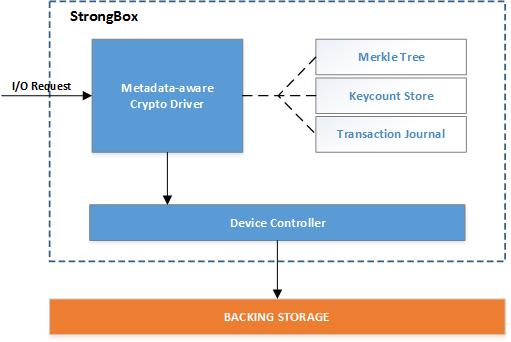
\includegraphics[width=1.0\linewidth]{overview.jpg}
   \caption{Overview of the \SYSTEM{} construction.}
    \label{fig:overview}
\end{figure}

\SYSTEM{}'s design is illustrated in \figref{overview}. \SYSTEM{}'s
metadata is encapsulated in three primary components: an in-memory
\emph{Merkle Tree} and two disk-backed byte arrays, the \emph{Keycount
  Store} and the \emph{Transaction Journal}. These components are
integrated into the \emph{Cryptographic Driver}, which is responsible
for handling data encryption, verification, and decryption during
interactions with the underlying backing store. These interactions
take place while fulfilling high-level I/O requests received from the
overlying LFS. Low-level I/O between \SYSTEM{} and the backing store
is handled by the \emph{Device Controller}.

The rest of this section describes the components referenced in
\figref{overview}. Specifically: we first describe the backing store
and \SYSTEM{}'s layout for data and metadata. This is followed by an
exploration of the cryptographic driver and how it interacts with that
metadata, the role of the device controller, an overview of rekeying
in the backing store, and further considerations to ensure
confidentiality in the case of rollbacks and related attacks.

\section{Backing Store Function and Layout}

% What is it?
The backing store is the storage media on which \SYSTEM{} operates.
\figref{backstore} illustrates \SYSTEM{}'s layout in the backing
store.

\begin{figure}[ht]
 \centering
  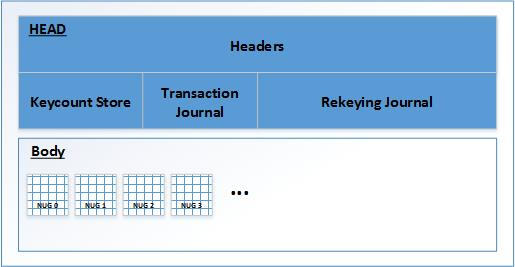
\includegraphics[width=1.0\linewidth]{backstore.jpg}
   \caption{Layout of \SYSTEM{}'s backing storage.}
    \label{fig:backstore}
\end{figure}

% Why is it a thing?
In the \textit{Body} section of the backing store layout, end-user
data is partitioned into a series of same-size logical
\emph{blocks}---distinct from the concept of physical disk blocks,
which are collections of one or more disk sectors. To make this
distinction clear, we refer to these wider logical blocks as
\emph{nuggets}, marked \textit{NUG} in the Body section of
\figref{backstore}. Hence, a nugget consists of one or more physical
disk blocks, depending on its configured size. Each nugget is
subdivided into a constant number of sub-blocks we refer to as
\emph{flakes}. \PUNT{The size of each flake and the number of flakes
  per nugget is configured by the user when \SYSTEM{} is initialized.}

The reason for these nugget/flake divisions are two-fold:
\begin{enumerate}
\item To limit the maximum length of any plaintexts operated on by the
  cryptographic driver, decreasing the overhead incurred per I/O
  operation and
\item To track, detect, and handle overwrites in the backing store.
\end{enumerate}

% Describe how the components in fig 1 are represented on disk and how
% they play into the overall design WITHOUT naming them
Hence, we must keep track of writes so that we may detect when an
overwrite occurs. Flakes are key to this tracking. When a request
comes in to write to one or more flakes in a nugget, \SYSTEM{} marks
the affected flakes ``dirty''. Here, dirty implies that another write
to some portion of that flake would constitute an overwrite. If a new
request comes in to write to one or more of those same flakes another
time, \SYSTEM{} triggers a rekeying procedure over the entire nugget
to safely overwrite the old data in those flakes. This rekeying
procedure is necessarily time consuming, adding to the overhead of
overwrites translated by \SYSTEM{}.

The \textit{head} section of the backing store contains the headers,
which are the metadata written to disk during \SYSTEM{}
initialization. These headers govern \SYSTEM{} operation and are, in
order:
\begin{enumerate}
\item VERSION, 4 bytes; specifies the \SYSTEM{} version originally
  used to initialize the backing store
\item SALT, 16 bytes; the salt used in part to derive the global
  master secret
\item MTRH, 32 bytes; the hash output of the Merkle Tree root
\item TPMGLOBALVER, 8 bytes; the monotonic global version count; also
  stored hardware-supported secure storage
\item VERIFICATION, 32 bytes; used to determine if the key derived
  from a password is correct
\item NUMNUGGETS, 4 bytes; the number of nuggets contained by the
  backing store
\item FLAKESPERNUGGET, 4 bytes; the number of flakes per nugget
\item FLAKESIZE, 4 bytes; the size on disk of each flake, in bytes
\item INITIALIZED, 1 byte; used to determine if the backing store has
  been properly initialized
\item REKEYING, 4 bytes; the index of the nugget in need of rekeying
  if there is a pending rekeying procedure
\end{enumerate}

After the headers, two byte arrays are stored in the Head section: an
array of $N$ 8-byte integer \textit{keycounts} and an array of $N$
$\ceil{P / 8}$-byte \textit{transaction journal entries}, where $N$ is
the number of nuggets in the backing store and $P$ is the number of
flakes per nugget.

Finally, the \emph{Rekeying Journal} is stored at the end of the Head
section.  The rekeying journal is where nuggets and their associated
metadata are transiently written, enabling \SYSTEM{} to recover to a
valid state in the event that it is interrupted during the rekeying
procedure.

\section{Metadata-aware Cryptographic Driver}

% What is it? Why is it a thing?
The cryptographic driver coordinates \SYSTEM{}'s disparate components.
Its primary function is to map incoming reads and writes to their
proper destinations in the backing store, applying our chosen stream
cipher and message authentication code to encrypt, verify, and decrypt
data on the fly with consideration for metadata management.

When a read request is received, it is first partitioned with respect
to affected nuggets; \ie{} a read that spans two nuggets would be
partitioned in half. For each nugget affected, we calculate which
flakes are touched by the request. We then verify the contents of
those flakes. If all the flakes are valid, whatever subset of data
that was requested by the user is decrypted and returned.
\algoref{read} details \SYSTEM{}'s read operation.

Like reads, when a write request is received, the request is first
partitioned with respect to affected nuggets. For each affected
nugget, we calculate which flakes are touched by the request and then
check if any of those flakes are marked as dirty in the transaction
journal. If one or more of them have been marked dirty, we trigger
rekeying for this specific nugget (see: \algoref{rekeying}) and end
there. Otherwise, we mark these touched flakes as dirty in the
transaction journal. We then iterate over these touched flakes. For
the first and last flakes touched by the write request, we execute an
internal read request (see: \algoref{read}) to both obtain the flake
data and verify that data with the Merkle Tree. We then overwrite
every touched flake with the data from the requested operation, update
the Merkle Tree to reflect this change, encrypt and write out the new
flake data, and commit all corresponding metadata. \algoref{write}
details \SYSTEM{}'s write operation.

\begin{algorithm}[h]
\floatname{algorithm}{CryptedRead (Algorithm 1)}
\caption{\SYSTEM{} in operating mode: handling an incoming read request.}
\label{algo:read}
\begin{algorithmic}[1]
\Require The read request is taken over a contiguous segment of the backing
store
\Require $\ell, \ell' \leftarrow$ read requested length
\Require $\aleph \leftarrow$ master secret
\Require $n_{index} \leftarrow$ first nugget index to be read
\State $data \leftarrow$ \emph{empty}
\While{$\ell \neq 0$}
    \State $k_{n_{index}} \leftarrow GenKey_{nugget}(n_{index}, \aleph)$
    \State Fetch nugget keycount $n_{kc}$ from Keycount Store.
    \State Calculate indices touched by request: $f_{first}$, $f_{last}$
    \State $n_{flakedat} \leftarrow ReadFlakes(f_{first},\dots,f_{last})$
    \For{$f_{current} = f_{first}$ \textbf{to} $f_{last}$}
        \State $k_{f_{current}} \leftarrow GenKey_{flake}(k_{n_{index}},
        f_{current}, n_{kc})$
        \State $tag_{f_{current}} \leftarrow GenMac(k_{f_{current}},
        n_{flakedat}[f_{current}])$
        \State Verify $tag_{f_{current}}$ in Merkle Tree.
    \EndFor 
    \LineComment{(\textbf{*}) denotes requested subset of nugget data}
    \State $data \leftarrow data + Decrypt(*n_{flakedat}, k_{n_{index}},
    n_{kc})$
    \State $\ell \leftarrow \ell - \|*n_{flakedat}\|$
    \State $n_{index} \leftarrow n_{index} + 1$
\EndWhile 
\\\Return $data$ \Comment{Fulfill the read request}
\Ensure $\|data\| <= \ell'$ 
\Ensure $\ell = 0$
\vskip -1.5em
\end{algorithmic}
\end{algorithm}

\begin{algorithm}[h]
\floatname{algorithm}{CryptedWrite (Algorithm 2)}
\caption{\SYSTEM{} in operating mode: handling an incoming write request.}
\label{algo:write}
\begin{algorithmic}[1]
\Require The write request applies to a contiguous segment of the backing store
\Require $\ell, \ell' \leftarrow$ write requested length
\Require $\aleph \leftarrow$ master secret
\Require $data \leftarrow$ cleartext data to be written
\Require $n_{index} \leftarrow$ first nugget index to be affected
\While{$\ell \neq 0$}
    \State Calculate indices touched by request: $f_{first}$, $f_{last}$
    \If{Transaction Journal entries for $f_{first},\dots,f_{last} \neq 0$}
        \State Trigger rekeying procedure (see: \algoref{rekeying}).
        \State \textbf{continue}
    \EndIf 
    \State Set Transaction Journal entries for $f_{first},\dots,f_{last}$ to 1
    \State $k_{n_{index}} \leftarrow GenKey_{nugget}(n_{index}, \aleph)$
    \State Fetch nugget keycount $n_{kc}$ from Keycount Store.
    \For{$f_{current} = f_{first}$ \textbf{to} $f_{last}$}
        \State $n_{flakedat} \leftarrow $ \textit{empty}
        \If{$f_{current} == f_{first} \| f_{current} == f_{last}$}
            \State $n_{flakedat} \leftarrow CryptedRead(\textit{FSIZE}, \aleph,
            n_{index}$@$f_{offset})$
        \EndIf 
        \State $n_{flakedat} \leftarrow Encrypt(n_{flakedat}, k_{n_{index}},
        n_{kc})$
        \State $k_{f_{current}} \leftarrow GenKey_{flake}(k_{n_{index}},
        f_{current}, n_{kc})$
        \State $tag_{f_{current}} \leftarrow GenMac(k_{f_{current}},
        n_{flakedat})$
        \State Update new $tag_{f_{current}}$ in Merkle Tree.
        \State $WriteFlake(f_{current}, n_{flakedat})$
        \\\LineComment{(\textbf{*}) denotes requested subset of nugget data if
        applicable}
        \State $\ell \leftarrow \ell - \|*n_{flakedat}\|$
    \EndFor 
    \State $n_{index} \leftarrow n_{index} + 1$
\EndWhile 
\State Update and commit metadata and headers
\Ensure $\ell = 0$
\vskip -1.5em
\end{algorithmic}
\end{algorithm}

% Algorithmic analysis?

\subsection{Transaction Journal}

An overwrite in \SYSTEM{} breaks the security guarantee offered by
any stream cipher. To prevent this failure, incoming write requests
must be tracked to ensure that overlapping writes do not occur. This
tracking is done with the transaction journal, featured in
\figref{overview}.

% Describe how this component meets that need
The transaction journal consists of $N$ $\ceil{P / 8}$-byte bit
vectors where $N$ is the number of nuggets in the backing store and
$P$ is the number of flakes per nugget. A bit vector $v$ contains at
least $P$ bits $v = \{ b_0, b_1, b_2, \dots, b_{P-1}, \dots \}$, with
extra bits ignored. Each vector is associated with a nugget and each
bit is associated with a flake belonging to that nugget.  When an
incoming write request occurs that affects several flakes in a nugget,
the corresponding bit vector is updated (set to 1) to reflect the new
dirty state of those flakes.

% Describe briefly TJ's relation to writes: when it's referenced and when it's
% changed
The transaction journal is referenced during each write request, where
it is updated to reflect the state of the nugget and checked to ensure
the operation does not constitute an overwrite. If the operation
\textit{does} constitute an overwrite, \SYSTEM{} triggers a rekeying
procedure for the entire nugget before safely completing the request.

\subsection{Merkle Tree}

% Brief recap of integrity protection and why it's important/a thing
Tracking writes with the transaction journal may stymie a passive
attacker by preventing explicit overwrites, but a sufficiently
motivated active attacker could resort to all manner of cut-and-paste
tactics with nuggets, flakes, and even blocks and sectors. If, for
example, an attacker purposefully zeroed-out the transaction journal
entry pertaining to a specific nugget in some out-of-band
manner---such as when \SYSTEM{} is shut down and then later
re-initialized with the same backing store---\SYSTEM{} would consider
any successive incoming writes as if the nugget were in a completely
clean state, even though it actually is not. This attack would force
\SYSTEM{} to make compromising overwrites. To prevent such attacks, we
must ensure that the backing store is always in a valid state. More
concretely: we must provide an integrity guarantee on top of a
confidentiality guarantee.

\SYSTEM{} uses our chosen MAC algorithm and each flake's unique key to
generate a per-flake MAC tag. Each tag is then appended to the Merkle
Tree along with \SYSTEM{}'s metadata. The transaction journal entries
are handled specially in that the bit vectors are MACed and the result
is appended to the Merkle Tree.  This is done to save space.

% Describe Merkle Tree's relation to writes and when it's checked
\PUNT{When \SYSTEM{} receives an I/O request, any flakes affected by the
request are validated in the Merkle Tree before the data is crypted
and the request fulfilled. On handling writes specifically, \SYSTEM{}
updates the Merkle Tree with the new data, updates any associated
metadata, and then calculates and commits the new root hash of the
Merkle Tree to the MTRH header in the backing store. In our
implementation, if there is a verification failure at this point, the
requested operation will fail and the process will shut down.

When \SYSTEM{} is first initialized, it constructs a fresh Merkle Tree
over the backing store's contents and compares the calculated root
hash with the MTRH header read in from the backing store. In our
implementation, if these values do not match, the user is notified
that the data integrity check failed.  They must then manually force
\SYSTEM{} to initialize with the compromised backing store.}

\subsection{Keycount Store}

% What is it?
To prevent a many-time pad attack, each nugget is assigned its own
form of nonce we refer to as a \emph{keycount}. The keycount store in
\figref{overview} represents a byte-array containing $N$ 8-byte
integer keycounts indexed to each nugget.  Along with acting as the
per-nugget nonce consumed by the stream cipher, the keycount is used
to derive the per-flake unique subkeys used in MAC tag generation.

\subsection{Rekeying Procedure}

% What is this? Why is this necessary?
When a write request would constitute an overwrite, \SYSTEM{} will
trigger a rekeying process instead of executing the write normally.
This rekeying process allows the write to proceed without causing a
catastrophic confidentiality violation.

% How does it work?
When rekeying begins, the nugget in question is loaded into memory and
decrypted. The target data is written into its proper offset in this decrypted
nugget. The nugget is then encrypted, this time with a different nonce
(\textit{keycount + 1}), and written to the backing store, replacing the
outdated nugget data. See: \algoref{rekeying}.

\begin{algorithm}[h]
\floatname{algorithm}{Rekeying (Algorithm 3)}
\caption{\SYSTEM{} rekeying process.}
\label{algo:rekeying}
\begin{algorithmic}[1]
\Require The original write request applied to a contiguous segment of the
backing store
\Require $\ell \leftarrow$ write requested length
\Require $\aleph \leftarrow$ master secret
\Require $data \leftarrow$ cleartext data to be written
\Require $n_{index} \leftarrow$ nugget rekeying target

\Comment{Read in and decrypt the entire nugget}
\State $n_{nuggetdat} \leftarrow CryptedRead(\textit{NSIZE}, \aleph, n_{index})$
\State Calculate indices touched by request: $f_{first}$, $f_{last}$
\State Write $data$ into $n_{nuggetdat}$ at proper offset with length $\ell$
\State Set Transaction Journal entries for $f_{first},\dots,f_{last}$ to 1
\State $k_{n_{index}} \leftarrow GenKey_{nugget}(n_{index}, \aleph)$
\State Fetch nugget keycount $n_{kc}$ from Keycount Store. Increment it by one.
\State $n_{nuggetdat} \leftarrow Encrypt(n_{nuggetdat}, k_{n_{index}}, n_{kc})$
\State Commit $n_{nuggetdat}$ to the backing store

\Comment{Iterate over all flakes in the nugget}
\ForAll{flakes $f_{current}$ \textbf{in} $n_{index}$}
    \State $k_{f_{current}} \leftarrow GenKey_{flake}(k_{n_{index}},
    f_{current}, n_{kc})$
    \State Copy $f_{current}$ data from $n_{nuggetdat} \rightarrow n_{flakedat}$
    \State $tag_{f_{current}} \leftarrow GenMac(k_{f_{current}}, n_{flakedat})$
    \State Update new $tag_{f_{current}}$ in Merkle Tree.
\EndFor 
\State Update and commit metadata and headers
\vskip -1.5em
\end{algorithmic}
\end{algorithm}

\section{Defending Against Rollbacks: Global Version Counter}

% The TPM and Trust Zone, what rollbacks are and how they're just as bad as
% overwrites
To prevent \SYSTEM{} from making overwrites, the status of each flake
is tracked and overwrites trigger a rekeying procedure. Tracking flake
status alone is not enough, however. An attacker could take a snapshot
of the backing store in its current state and then easily rollback to
a previously valid state. At this point, the attacker could have
\SYSTEM{} make writes that it does not recognize as overwrites.

With AES-XTS, the threat posed by rolling the backing store to a
previously valid state is outside of its threat model. Despite this,
data confidentiality guaranteed by AES-XTS holds in the event of a
rollback, even if integrity is violated.

\SYSTEM{} uses a monotonic global version counter to detect rollbacks.
In the case that a rollback is detected, \SYSTEM{} will refuse to
initialize without warning. Whenever a write request is completed,
this global version counter is committed to the backing store,
committed to secure hardware, and updated in the in-memory Merkle
Tree.

%\TODO{We need a to talk about TPM/TZ ``burnout'' from many overwrites as Ari
%described.}

\chapter{\SYSTEM{} Implementation} \label{sec:implementation}

Our implementation of \SYSTEM{} is comprised of 5000 lines of C code. Libraries
used by \SYSTEM{} include OpenSSL version 1.0.2 and LibSodium version 1.0.12 for
its ChaCha20, Argon2, Blake2, and AES-XTS implementations. The SHA-256 Merkle
Tree implementation is borrowed from the Secure Block Device library~\cite{SBD}.
The implementation is available at https://github.com/ananonrepo2/StrongBox.

To reduce the complexity of the experimental setup and allow \SYSTEM{}
to run in user space, we provide a virtual device interface through
the BUSE~\cite{BUSE} virtual block device layer, itself based on the
Network Block Device (NBD).

\section{Deriving Subkeys}
To function, the cryptographic driver must be made aware of a shared
master secret. The method of derivation of this master secret is
implementation specific and has no impact on performance as it is
completed during \SYSTEM{}'s initialization. Our implementation of
\SYSTEM{} utilizes the Argon2 KDF to derive a master secret from a
given password with an acceptable time-memory trade-off.

% Describe deriving the nugget keys from the master secret
To assign each nugget its own unique keystream, that nugget requires a
unique key and associated nonce. Our implementation of \SYSTEM{}
derives these nugget subkeys from the master secret during \SYSTEM{}'s
initialization. To guarantee the backing store's integrity, each flake
is tagged with a MAC. Our implementation of \SYSTEM{} uses Poly1305,
accepting a 32-byte one-time key and a plaintext of arbitrary length
to generate tags. These one-time flake subkeys are derived from their
respective nugget subkeys.

\section{A Secure, Persistent Counter} 

Our target platform uses an embedded Multi-Media Card (eMMC) as a backing store. In
addition to boot and user data partitions, the eMMC standard includes a secure storage
partition called a Replay Protected Memory Block (RPMB)~\cite{eMMC-standard}. The RPMB
partition's size is fixed at manufacturing time, and all read and write commands issued
to it must be authenticated by a key that is fixed when the device is first set up.

To implement rollback protection on top of the RPMB, the key for authenticating RPMB
commands could be sealed in TEE sealed storage so that it would only be accessible to a
specific enclave running in a TEE. This enclave would be responsible for reading and
writing the \SYSTEM{} global version counter to the RPMB, and enforcing that invariant
that it only increase monotonically. Our design is not dependent on the eMMC standard,
however. Other trusted hardware mechanisms, including TPMs, support secure, persistent
storage or monotonic counters that could be adapted for use with \SYSTEM{}.

There are two practical concerns we must address for implementing the
secure counter: wear and performance overhead.  Wear is a concern because the
counter is implemented in non-volatile storage.  The RPMB implements
all the same wear protection mechanisms that are used to store
user-data~\cite{eMMC-standard}.  In addition, \SYSTEM{} writes to the
global version counter once per write to user-data.  Given that the
eMMC implements the same wear protection for the RPMB and user data,
and that the ratio of writes to these areas is 1:1, we expect
\SYSTEM{} places no additional wear burden on the hardware.  In terms
of performance overhead, updating the global version counter requires
making one 64-bit authenticated write per user-data write.  As
user-data writes will almost always be substantially larger, we
anticipate no significant overhead from the using the RPMB to store
the secure counter.

\section{LFS Garbage Collection}

% What is this? Why is this necessary?
An LFS attempts to write to a disk sequentially and in an append-only fashion,
as if it were writing to a log. This requires large amounts of contiguous space
on disk, called \emph{segments}. Since any backing store is necessarily finite
in capacity, an LFS can only append so much data before it runs out of free
space. When this occurs, the LFS triggers a \emph{segment cleaning algorithm} to
erase any outdated data and compress the remainder of the log down into as few
segments as possible~\cite{LFS,F2FS}. This segment cleaning procedure is known
more broadly as \emph{garbage collection}~\cite{F2FS}.

In the context of \SYSTEM{}, garbage collection could potentially
incur high overhead. The procedure itself would, with its every write,
require a rekeying of any affected nuggets. Worse, every proceeding
write would appear to \SYSTEM{} as if it were an overwrite, since
there is no way for \SYSTEM{} to know that the LFS triggered garbage
collection internally.

In practice, modern production LFSes are optimized to perform garbage collection
as few times as possible~\cite{F2FS}. Further, they often perform garbage
collection in a background thread that triggers when the filesystem is idle and
only perform expensive on-demand garbage collection when the backing store is
nearing capacity~\cite{F2FS, NILFS}. We leave garbage collection turned on for
all of our tests and see no substantial performance degradation from this
process because it is scheduled not to interfere with user I/O.

\chapter{Evaluation} \label{sec:evaluation}

\section{Experimental Setup}

We implement a prototype of \SYSTEM{} on a Hardkernel Odroid XU3 ARM big.LITTLE
system (Samsung Exynos5422 A15 and A7 quad core CPUs, 2Gbyte LPDDR3 RAM, eMMC5.0
HS400 backing store) running Ubuntu Trusty 14.04 LTS, kernel version 3.10.58. 
% We use the energymon portable interface~\cite{energymon} to measure
% instantaneous energy and power consumption by polling the odroid's
% internal INA-231 power sensors.

\section{Experimental Results}

In this section we seek to answer four questions:
\begin{enumerate}
\item What is \SYSTEM{}'s overhead when compared to dm-crypt AES-XTS?
\item How does the \SYSTEM{} under an LFS (\ie F2FS) configuration compare to
the popular dm-crypt under Ext4 configuration?
\item Where does \SYSTEM{} derive its performance gains? Implementation? Choice
of cipher?
\item How does \SYSTEM{} perform when the backing store is nearly full?
\end{enumerate}

To evaluate the performance of \SYSTEM{}, we measure the latency
(seconds/milliseconds per operation) of both sequential and random read and
write I/O operations across four different standard Linux filesystems: NILFS2,
F2FS, Ext4 in ordered journaling mode, and Ext4 in full journaling mode. The I/O
operations are performed using file sizes between 4KB and 40MB. These files
were populated with random data; this data remained constant throughout the
evaluation. The experiments were performed using a standard Linux ramdisk
(tmpfs) as the ultimate backing store.

Ext4 ordered journaling mode (\texttt{data=ordered}) is the default mode of
Ext4, where metadata is committed to the filesystem's journal while
the actual data is written through to the main filesystem. In the event of a
crash, the filesystem can use the journal to avoid damage and recover to a
consistent state. Full journaling mode (\texttt{data=journal}) journals both
metadata and the filesystem's actual data---essentially a double write-back for
each write operation. In the event of a crash, the journal can be used to replay
entire I/O events so that both the filesystem and its data can be recovered. We
include both modes of Ext4 to further explore the impact of frequent overwrites
against \SYSTEM{}.

The experiment consists of reading and writing each file in its entirety 30
times sequentially, and then reading and writing random portions of each file 30
times. In both cases, the same amount of data was read and written per file. The
median latency was taken per result set. We chose 30 read/write operations (10
read/write operations repeated three times each) to handle potential variation.
The Linux page cache was dropped before every read operation, each file was
opened in synchronous I/O mode via \texttt{O\_SYNC}, and we relied on non-
buffered \texttt{read()}/\texttt{write()} system calls. A high-level I/O size of
128KB was used for all read and write calls that hit the filesystems; however,
the I/O requests being made at the block device layer varied between 4KB and
128KB depending on the filesystem under test.

The experiment was repeated on each filesystem in three different
configurations:

\begin{enumerate}
\item \textit{unencrypted}: Filesystem mounted atop a BUSE virtual block
  device set up to immediately pass through any incoming I/O requests straight
  to the backing store. We use this as the baseline measurement of the
  filesystem's performance without any encryption.
\item \textit{\SYSTEM{}}: Filesystem mounted atop a BUSE virtual block
  device provided by our \SYSTEM{} implementation to perform full-disk
  encryption.
\item \textit{dm-crypt}: Filesystem mounted atop a Device Mapper
 ~\cite{LinuxDeviceMapper} higher-level virtual block device provided by
  dm-crypt to perform full-disk encryption, which itself is mounted atop a
  BUSE virtual block device with pass through behavior identical to the device
  used in the baseline configuration. dm-crypt was configured to use AES-XTS as
  its full-disk encryption algorithm. All other parameters were left at their
  default values.
\end{enumerate}

\figref{microbench-f2fs} compares \SYSTEM{} to dm-crypt under the F2FS
filesystem.  The gamut of result sets over different filesystems can
be seen in \figref{microbench-gamut}.  \figref{microbench-ext4}
compares Ext4 with dm-crypt to F2FS with \SYSTEM{}.  

\begin{figure}[ht]
    \textbf{\SYSTEM{} vs dm-crypt AES-XTS: F2FS Test}\par\medskip
    \centering
    \begin{subfigure}{0.5\linewidth}
        \centering
        {\begin{tikzpicture}[baseline]

\definecolor{s1}{RGB}{225, 175, 0}
\definecolor{s2}{RGB}{245, 30, 28}
\definecolor{s3}{RGB}{175, 60, 175}
\definecolor{s4}{RGB}{26, 228, 28}
\definecolor{s5}{RGB}{26, 163, 152}
\definecolor{s6}{RGB}{225, 128, 0}

\pgfkeys{
    /pgf/number format/precision=1, 
    /pgf/number format/fixed zerofill=true
}

\pgfplotsset{
    nodes near coords greater equal only/.style={
        small value/.style={
            /tikz/coordinate,
        },
        every node near coord/.append style={
            check for small values/.code={
                \begingroup
                \pgfkeys{/pgf/fpu}
                \pgfmathparse{\pgfplotspointmeta<#1}
                \global\let\result=\pgfmathresult
                \endgroup
                \pgfmathfloatcreate{1}{1.0}{0}
                \let\ONE=\pgfmathresult
                \ifx\result\ONE
                    \pgfkeysalso{/pgfplots/small value}
                \fi
            },
            check for small values
        },
    },
}

\pgfmathsetmacro{\ymax}{4}
\pgfmathsetmacro{\height}{6cm}

\begin{groupplot}[
    group style={
        group name=plots,
        group size=1 by 1,
        xlabels at=edge top,
        xticklabels at=edge top,
        vertical sep=5pt
    },
    axis x line*=top,
    xlabel near ticks,
    major x tick style=transparent,
    height=\height,
    width=\columnwidth,
    xmin=0, xmax=5,
    % enlarge y limits={value=0.2,upper},
    tick align=outside,
    tick style={white},
    ytick=\empty,
    xtick=\empty,
    xticklabels={},
    yticklabels={},
    % restrict y to domain*=0:2,
]
\nextgroupplot[
    ylabel={\footnotesize Latency (normalized to unencrypted)},
    ylabel shift={6mm},
    ymin=0, ymax=1,
]
\end{groupplot}

\begin{groupplot}[
    group style={
        group name=plots,
        group size=1 by 1,
        xlabels at=edge bottom,
        xticklabels at=edge bottom,
        vertical sep=5pt,
        horizontal sep=15cn
    },
    axis x line*=bottom,
    xlabel near ticks,
    major x tick style=transparent,
    height=\height,
    width=\linewidth,
    xmin=0, xmax=2,
    tick align=outside,
    tick style={ black },
    xlabel={\footnotesize File Size (bytes)},
    xtick={ 0, 0.3, 0.65, 1.0, 1.35, 1.7, 2 },
    xticklabels={ , 4K , 512K , 5M , 40M , Mean, },
    ymin=1, ymax=\ymax,
    % restrict y to domain*=0:2,
    ytick={ 1, 2, 3, 4 },
    yticklabels={ 1, 2, 3, 4 },
    extra y ticks={ 1.5, 2.5, 3.5 },
    extra y tick style={grid=minor, grid style={dotted, gray}},
    extra y tick label=\empty,
    % enlarge y limits={value=0.2,upper},
    legend cell align=center,
    legend style={ column sep=1ex },
    ymajorgrids=true,
    grid style=\empty,
    every node near coord/.append style={font=\tiny},
    % stackoverflow magic to make the numbers appear above the overly long bars
    visualization depends on={rawy \as \rawy},
    nodes near coords={\pgfmathprintnumber\rawy},
    restrict y to domain*={
        \pgfkeysvalueof{/pgfplots/ymin}:\pgfkeysvalueof{/pgfplots/ymax}
    },
    nodes near coords greater equal only=\ymax,
]
\nextgroupplot[
    ybar=\pgflinewidth,
    bar width=4.5pt,
    legend entries={
        {\scriptsize StrongBox/reads},
        {\scriptsize dm-crypt/reads},
        {\scriptsize StrongBox/writes},
        {\scriptsize dm-crypt/writes},
    },
    legend style={
        draw=none,
        legend columns=2,
        at={(0.525,1.35)},
        anchor=north
    },
]

\addplot[fill=s5, every node near coord/.append style={color=s5}] table[x index=0, y index=1, col sep=space] {img/microbench-f2fs-sequential.dat};
\addplot[fill=s2, every node near coord/.append style={color=s2}] table[x index=0, y index=2, col sep=space] {img/microbench-f2fs-sequential.dat};
\addplot[draw=s5, pattern=crosshatch, pattern color=s5, every node near coord/.append style={color=s5}] table[x index=0, y index=3, col sep=space] {img/microbench-f2fs-sequential.dat};
\addplot[draw=s2, pattern=crosshatch, pattern color=s2, every node near coord/.append style={color=s2}] table[x index=0, y index=4, col sep=space] {img/microbench-f2fs-sequential.dat};

\addplot[fill=s5, every node near coord/.append style={color=s5}] table[x index=0, y index=5, col sep=space] {img/microbench-f2fs-sequential.dat};
\addplot[fill=s5, every node near coord/.append style={color=s5}] table[x index=0, y index=6, col sep=space] {img/microbench-f2fs-sequential.dat};
\addplot[fill=s5, every node near coord/.append style={color=s5}] table[x index=0, y index=6, col sep=space] {img/microbench-f2fs-sequential.dat};

\addplot[fill=s5, every node near coord/.append style={color=s5}] table[x index=0, y index=7, col sep=space] {img/microbench-f2fs-sequential.dat};
\addplot[fill=s2, every node near coord/.append style={color=s2}] table[x index=0, y index=8, col sep=space] {img/microbench-f2fs-sequential.dat};
\addplot[draw=s5, pattern=crosshatch, pattern color=s5, every node near coord/.append style={color=s5}] table[x index=0, y index=9, col sep=space] {img/microbench-f2fs-sequential.dat};
\addplot[draw=s2, pattern=crosshatch, pattern color=s2, every node near coord/.append style={color=s2}] table[x index=0, y index=10, col sep=space] {img/microbench-f2fs-sequential.dat};

\addplot[fill=s5, every node near coord/.append style={color=s5}] table[x index=0, y index=11, col sep=space] {img/microbench-f2fs-sequential.dat};
\addplot[fill=s5, every node near coord/.append style={color=s5}] table[x index=0, y index=12, col sep=space] {img/microbench-f2fs-sequential.dat};
\addplot[fill=s5, every node near coord/.append style={color=s5}] table[x index=0, y index=12, col sep=space] {img/microbench-f2fs-sequential.dat};

\addplot[fill=s5, every node near coord/.append style={color=s5}] table[x index=0, y index=13, col sep=space] {img/microbench-f2fs-sequential.dat};
\addplot[fill=s2, every node near coord/.append style={color=s2}] table[x index=0, y index=14, col sep=space] {img/microbench-f2fs-sequential.dat};
\addplot[draw=s5, pattern=crosshatch, pattern color=s5, every node near coord/.append style={color=s5}] table[x index=0, y index=15, col sep=space] {img/microbench-f2fs-sequential.dat};
\addplot[draw=s2, pattern=crosshatch, pattern color=s2, every node near coord/.append style={color=s2}] table[x index=0, y index=16, col sep=space] {img/microbench-f2fs-sequential.dat};

\addplot[fill=s5, every node near coord/.append style={color=s5}] table[x index=0, y index=17, col sep=space] {img/microbench-f2fs-sequential.dat};
\addplot[fill=s5, every node near coord/.append style={color=s5}] table[x index=0, y index=18, col sep=space] {img/microbench-f2fs-sequential.dat};
\addplot[fill=s5, every node near coord/.append style={color=s5}] table[x index=0, y index=18, col sep=space] {img/microbench-f2fs-sequential.dat};

\addplot[fill=s5, every node near coord/.append style={color=s5}] table[x index=0, y index=19, col sep=space] {img/microbench-f2fs-sequential.dat};
\addplot[fill=s2, every node near coord/.append style={color=s2}] table[x index=0, y index=20, col sep=space] {img/microbench-f2fs-sequential.dat};
\addplot[draw=s5, pattern=crosshatch, pattern color=s5, every node near coord/.append style={color=s5}] table[x index=0, y index=21, col sep=space] {img/microbench-f2fs-sequential.dat};
\addplot[draw=s2, pattern=crosshatch, pattern color=s2, every node near coord/.append style={color=s2}] table[x index=0, y index=22, col sep=space] {img/microbench-f2fs-sequential.dat};

\addplot[fill=s5, every node near coord/.append style={color=s5}] table[x index=0, y index=23, col sep=space] {img/microbench-f2fs-sequential.dat};
\addplot[fill=s5, every node near coord/.append style={color=s5}] table[x index=0, y index=24, col sep=space] {img/microbench-f2fs-sequential.dat};
\addplot[fill=s5, every node near coord/.append style={color=s5}] table[x index=0, y index=24, col sep=space] {img/microbench-f2fs-sequential.dat};

\addplot[fill=s5, every node near coord/.append style={color=s5}] table[x index=0, y index=25, col sep=space] {img/microbench-f2fs-sequential.dat};
\addplot[fill=s2, every node near coord/.append style={color=s2}] table[x index=0, y index=26, col sep=space] {img/microbench-f2fs-sequential.dat};
\addplot[draw=s5, pattern=crosshatch, pattern color=s5, every node near coord/.append style={color=s5}] table[x index=0, y index=27, col sep=space] {img/microbench-f2fs-sequential.dat};
\addplot[draw=s2, pattern=crosshatch, pattern color=s2, every node near coord/.append style={color=s2}] table[x index=0, y index=28, col sep=space] {img/microbench-f2fs-sequential.dat};
\end{groupplot}%
\end{tikzpicture}%
}
        \caption{Sequential I/O expanded F2FS result set.}
        \label{fig:microbench-f2fs-sequential}
    \end{subfigure}\hspace*{0.5em}%
    \begin{subfigure}{0.5\linewidth}
        \centering
        \vspace{2em}
        {\begin{tikzpicture}[baseline]

\definecolor{s1}{RGB}{225, 175, 0}
\definecolor{s2}{RGB}{245, 30, 28}
\definecolor{s3}{RGB}{175, 60, 175}
\definecolor{s4}{RGB}{26, 228, 28}
\definecolor{s5}{RGB}{26, 163, 152}
\definecolor{s6}{RGB}{225, 128, 0}

\pgfkeys{
    /pgf/number format/precision=1, 
    /pgf/number format/fixed zerofill=true
}

\pgfplotsset{
    nodes near coords greater equal only/.style={
        small value/.style={
            /tikz/coordinate,
        },
        every node near coord/.append style={
            check for small values/.code={
                \begingroup
                \pgfkeys{/pgf/fpu}
                \pgfmathparse{\pgfplotspointmeta<#1}
                \global\let\result=\pgfmathresult
                \endgroup
                \pgfmathfloatcreate{1}{1.0}{0}
                \let\ONE=\pgfmathresult
                \ifx\result\ONE
                    \pgfkeysalso{/pgfplots/small value}
                \fi
            },
            check for small values
        },
    },
}

\pgfmathsetmacro{\ymax}{4}
\pgfmathsetmacro{\height}{6cm}

\begin{groupplot}[
    group style={
        group name=plots,
        group size=1 by 1,
        xlabels at=edge top,
        xticklabels at=edge top,
        vertical sep=5pt
    },
    axis x line*=top,
    xlabel near ticks,
    major x tick style=transparent,
    height=\height,
    width=\columnwidth,
    xmin=0, xmax=5,
    % enlarge y limits={value=0.2,upper},
    tick align=outside,
    tick style={white},
    ytick=\empty,
    xtick=\empty,
    xticklabels={},
    yticklabels={},
    % restrict y to domain*=0:2,
]
\nextgroupplot[
    ylabel={\footnotesize Latency (normalized to unencrypted)},
    ylabel shift={6mm},
    ymin=0, ymax=1,
]
\end{groupplot}

\begin{groupplot}[
    group style={
        group name=plots,
        group size=1 by 1,
        xlabels at=edge bottom,
        xticklabels at=edge bottom,
        vertical sep=5pt
    },
    axis x line*=bottom,
    xlabel near ticks,
    major x tick style=transparent,
    height=\height,
    width=\linewidth,
    xmin=0, xmax=2,
    tick align=outside,
    tick style={ black },
    xlabel={\footnotesize File Size (bytes)},
    xtick={ 0, 0.3, 0.65, 1.0, 1.35, 1.7, 2 },
    xticklabels={ , 4K , 512K , 5M , 40M , Mean, },
    ymin=1, ymax=\ymax,
    % restrict y to domain*=0:2,
    ytick={ 1, 2, 3, 4 },
    yticklabels={ 1, 2, 3, 4 },
    extra y ticks={ 1.5, 2.5, 3.5 },
    extra y tick style={grid=minor, grid style={dotted, gray}},
    extra y tick label=\empty,
    % enlarge y limits={value=0.2,upper},
    legend cell align=center,
    legend style={ column sep=1ex },
    ymajorgrids=true,
    grid style=\empty,
    every node near coord/.append style={font=\tiny},
    % stackoverflow magic to make the numbers appear above the overly long bars
    visualization depends on={rawy \as \rawy},
    nodes near coords={\pgfmathprintnumber\rawy},
    restrict y to domain*={
        \pgfkeysvalueof{/pgfplots/ymin}:\pgfkeysvalueof{/pgfplots/ymax}
    },
    nodes near coords greater equal only=\ymax,
]
\nextgroupplot[
    ybar=\pgflinewidth,
    bar width=4.5pt,
    % legend entries={
    %     {\scriptsize NIlfs/reaDS},
    %     {\scriptsize NILFS/writes},
    %     {\scriptsize F2FS/reads},
    %     {\scriptsize F2FS/writes},
    %     {\scriptsize Ext4OJ/reads},
    %     {\scriptsize Ext4OJ/writes},
    %     {\scriptsize Ext4FJ/reads},
    %     {\scriptsize Ext4FJ/writes},
    % },
    % legend style={
    %     draw=none,
    %     legend columns=4,
    %     at={(0.45,1.3)},
    %     anchor=north
    % },
]

\addplot[fill=s5, every node near coord/.append style={color=s5}] table[x index=0, y index=1, col sep=space] {img/microbench-f2fs-random.dat};
\addplot[fill=s2, every node near coord/.append style={color=s2}] table[x index=0, y index=2, col sep=space] {img/microbench-f2fs-random.dat};
\addplot[draw=s5, pattern=crosshatch, pattern color=s5, every node near coord/.append style={color=s5}] table[x index=0, y index=3, col sep=space] {img/microbench-f2fs-random.dat};
\addplot[draw=s2, pattern=crosshatch, pattern color=s2, every node near coord/.append style={color=s2}] table[x index=0, y index=4, col sep=space] {img/microbench-f2fs-random.dat};

\addplot[fill=s5, every node near coord/.append style={color=s5}] table[x index=0, y index=5, col sep=space] {img/microbench-f2fs-random.dat};
\addplot[fill=s5, every node near coord/.append style={color=s5}] table[x index=0, y index=6, col sep=space] {img/microbench-f2fs-random.dat};
\addplot[fill=s5, every node near coord/.append style={color=s5}] table[x index=0, y index=6, col sep=space] {img/microbench-f2fs-random.dat};

\addplot[fill=s5, every node near coord/.append style={color=s5}] table[x index=0, y index=7, col sep=space] {img/microbench-f2fs-random.dat};
\addplot[fill=s2, every node near coord/.append style={color=s2}] table[x index=0, y index=8, col sep=space] {img/microbench-f2fs-random.dat};
\addplot[draw=s5, pattern=crosshatch, pattern color=s5, every node near coord/.append style={color=s5}] table[x index=0, y index=9, col sep=space] {img/microbench-f2fs-random.dat};
\addplot[draw=s2, pattern=crosshatch, pattern color=s2, every node near coord/.append style={color=s2}] table[x index=0, y index=10, col sep=space] {img/microbench-f2fs-random.dat};

\addplot[fill=s5, every node near coord/.append style={color=s5}] table[x index=0, y index=11, col sep=space] {img/microbench-f2fs-random.dat};
\addplot[fill=s5, every node near coord/.append style={color=s5}] table[x index=0, y index=12, col sep=space] {img/microbench-f2fs-random.dat};
\addplot[fill=s5, every node near coord/.append style={color=s5}] table[x index=0, y index=12, col sep=space] {img/microbench-f2fs-random.dat};

\addplot[fill=s5, every node near coord/.append style={color=s5}] table[x index=0, y index=13, col sep=space] {img/microbench-f2fs-random.dat};
\addplot[fill=s2, every node near coord/.append style={color=s2}] table[x index=0, y index=14, col sep=space] {img/microbench-f2fs-random.dat};
\addplot[draw=s5, pattern=crosshatch, pattern color=s5, every node near coord/.append style={color=s5}] table[x index=0, y index=15, col sep=space] {img/microbench-f2fs-random.dat};
\addplot[draw=s2, pattern=crosshatch, pattern color=s2, every node near coord/.append style={color=s2}] table[x index=0, y index=16, col sep=space] {img/microbench-f2fs-random.dat};

\addplot[fill=s5, every node near coord/.append style={color=s5}] table[x index=0, y index=17, col sep=space] {img/microbench-f2fs-random.dat};
\addplot[fill=s5, every node near coord/.append style={color=s5}] table[x index=0, y index=18, col sep=space] {img/microbench-f2fs-random.dat};
\addplot[fill=s5, every node near coord/.append style={color=s5}] table[x index=0, y index=18, col sep=space] {img/microbench-f2fs-random.dat};

\addplot[fill=s5, every node near coord/.append style={color=s5}] table[x index=0, y index=19, col sep=space] {img/microbench-f2fs-random.dat};
\addplot[fill=s2, every node near coord/.append style={color=s2}] table[x index=0, y index=20, col sep=space] {img/microbench-f2fs-random.dat};
\addplot[draw=s5, pattern=crosshatch, pattern color=s5, every node near coord/.append style={color=s5}] table[x index=0, y index=21, col sep=space] {img/microbench-f2fs-random.dat};
\addplot[draw=s2, pattern=crosshatch, pattern color=s2, every node near coord/.append style={color=s2}] table[x index=0, y index=22, col sep=space] {img/microbench-f2fs-random.dat};

\addplot[fill=s5, every node near coord/.append style={color=s5}] table[x index=0, y index=23, col sep=space] {img/microbench-f2fs-random.dat};
\addplot[fill=s5, every node near coord/.append style={color=s5}] table[x index=0, y index=24, col sep=space] {img/microbench-f2fs-random.dat};
\addplot[fill=s5, every node near coord/.append style={color=s5}] table[x index=0, y index=24, col sep=space] {img/microbench-f2fs-random.dat};

\addplot[fill=s5, every node near coord/.append style={color=s5}] table[x index=0, y index=25, col sep=space] {img/microbench-f2fs-random.dat};
\addplot[fill=s2, every node near coord/.append style={color=s2}] table[x index=0, y index=26, col sep=space] {img/microbench-f2fs-random.dat};
\addplot[draw=s5, pattern=crosshatch, pattern color=s5, every node near coord/.append style={color=s5}] table[x index=0, y index=27, col sep=space] {img/microbench-f2fs-random.dat};
\addplot[draw=s2, pattern=crosshatch, pattern color=s2, every node near coord/.append style={color=s2}] table[x index=0, y index=28, col sep=space] {img/microbench-f2fs-random.dat};
\end{groupplot}%
\end{tikzpicture}%
}
        \caption{Random I/O expanded F2FS result set.}
        \label{fig:microbench-f2fs-random}
    \end{subfigure}
    \caption{Test of the F2FS LFS mounted atop both dm-crypt and
      \SYSTEM{}; median latency of different sized whole file read and
      write operations normalized to unencrypted access. By harmonic
      mean, \SYSTEM{} is 1.6$\times$ faster than dm-crypt for reads
      and 1.2$\times$ faster for writes.}
    \label{fig:microbench-f2fs}
\end{figure}

\section{\SYSTEM{} Read Performance}

\figref{microbench-f2fs} shows the performance of \SYSTEM{} in comparison to
dm-crypt, both mounted with the F2FS filesystem. We see \SYSTEM{} improves on
the performance of dm-crypt's AES-XTS implementation across sequential and
random read operations on all file sizes. Specifically, $2.07\times$ for
sequential 40MB, $2.08\times$ for sequential 5MB, $1.85\times$ for sequential
512KB, and $1.03\times$ for sequential 4KB.

\figref{microbench-gamut} provides an expanded performance profile for
\SYSTEM{}, testing a gamut of filesystems broken down by workload file size. For
sequential reads across all filesystems and file sizes, \SYSTEM{} outperforms
dm-crypt. This is true even on the non-LFS Ext4 filesystems. Specifically, we
see read performance improvements over dm-crypt AES-XTS for 40MB sequential
reads of $2.02\times$ for NILFS, $2.07\times$ for F2FS, $2.09\times$ for Ext4 in
ordered journaling mode, and $2.06\times$ for Ext4 in full journaling mode. For
smaller file sizes, the performance improvement is less pronounced.
Specifically, for 4KB reads we see $1.28\times$ for NILFS, $1.03\times$ for
F2FS, $1.07\times$ for Ext4 in ordered journaling mode, and $1.04\times$ for
Ext4 in full journaling mode.

When it comes to random reads, we see virtually identical results save for 4KB
reads, where dm-crypt proved very slightly more performant under the NILFS
LFS at $1.12\times$. This behavior was not observed under the more modern F2FS
LFS.

\PUNT{These results demonstrate the claim from the introduction: under Log- structured
File Systems, \SYSTEM{} improves read performance over more traditional AES-XTS
based full disk encryption schemes by upwards of $2\times$ while maintaining a
confidentiality guarantee and additionally providing a data integrity guarantee.
Further, these results suggest that implementing a stream-cipher based full-disk
encryption scheme with added integrity protection is not so expensive as to make
it untenable. Indeed, we can achieve significant performance wins by leveraging
the speed of fast stream ciphers, especially on systems with a heavy read bias,
\ie web servers, media hosts, and some mobile devices.}


\begin{figure*}[t]
    \textbf{\SYSTEM{} Four Filesystems Test}\par\medskip
    \centering
    \begin{subfigure}{0.5\linewidth}
        \centering
        {\begin{tikzpicture}[baseline]

\definecolor{s1}{RGB}{225, 175, 0}
\definecolor{s2}{RGB}{245, 30, 28}
\definecolor{s3}{RGB}{175, 60, 175}
\definecolor{s4}{RGB}{26, 228, 28}
\definecolor{s5}{RGB}{26, 163, 152}
\definecolor{s6}{RGB}{225, 128, 0}

\pgfkeys{
    /pgf/number format/precision=1, 
    /pgf/number format/fixed zerofill=true
}

\pgfplotsset{
    nodes near coords greater equal only/.style={
        small value/.style={
            /tikz/coordinate,
        },
        every node near coord/.append style={
            check for small values/.code={
                \begingroup
                \pgfkeys{/pgf/fpu}
                \pgfmathparse{\pgfplotspointmeta<#1}
                \global\let\result=\pgfmathresult
                \endgroup
                \pgfmathfloatcreate{1}{1.0}{0}
                \let\ONE=\pgfmathresult
                \ifx\result\ONE
                    \pgfkeysalso{/pgfplots/small value}
                \fi
            },
            check for small values
        },
    },
}

\pgfmathsetmacro{\ymax}{2}

\begin{groupplot}[
    group style={
        group name=plots,
        group size=1 by 1,
        xlabels at=edge top,
        xticklabels at=edge top,
        vertical sep=5pt
    },
    axis x line*=top,
    xlabel near ticks,
    major x tick style=transparent,
    height=6cm,
    width=\columnwidth,
    xmin=0, xmax=5,
    % enlarge y limits={value=0.2,upper},
    tick align=outside,
    tick style={white},
    ytick=\empty,
    xtick=\empty,
    xticklabels={},
    yticklabels={},
    % restrict y to domain*=0:2,
]
\nextgroupplot[
    ylabel={\footnotesize Latency (normalized to dm-crypt)},
    ylabel shift={6mm},
    ymin=0, ymax=1,
]
\end{groupplot}

\begin{groupplot}[
    group style={
        group name=plots,
        group size=1 by 1,
        xlabels at=edge bottom,
        xticklabels at=edge bottom,
        vertical sep=5pt
    },
    axis x line*=bottom,
    xlabel near ticks,
    major x tick style=transparent,
    height=6cm,
    width=\columnwidth,
    xmin=0, xmax=2,
    tick align=outside,
    tick style={ black },
    xlabel={\footnotesize File Size (bytes)},
    xtick={ 0, 0.35, 0.75, 1.2, 1.625, 2 },
    xticklabels={ , \footnotesize{4K} , \footnotesize{512K} , \footnotesize{5M} , \footnotesize{40M}, },
    ymin=0, ymax=\ymax,
    % restrict y to domain*=0:2,
    ytick={ 0, 0.5, 1.5, 2 },
    yticklabels={ 0, 0.5, 1.5, 2 },
    extra y ticks={1},
    extra y tick style={grid=major, grid style={dashed, black}},
    extra y tick label={ 1 },
    % enlarge y limits={value=0.2,upper},
    legend cell align=center,
    legend style={ column sep=1ex },
    ymajorgrids=true,
    grid style={ dotted, gray },
    every node near coord/.append style={font=\tiny},
    % stackoverflow magic to make the numbers appear above the overly long bars
    visualization depends on={rawy \as \rawy},
    nodes near coords={\pgfmathprintnumber\rawy},
    restrict y to domain*={
        \pgfkeysvalueof{/pgfplots/ymin}:\pgfkeysvalueof{/pgfplots/ymax}
    },
    nodes near coords greater equal only=\ymax,
]
\nextgroupplot[
    ybar=\pgflinewidth,
    bar width=4.5pt,
    legend entries={
        {\scriptsize NILFS/reads},
        {\scriptsize F2FS/reads},
        {\scriptsize Ext4OJ/reads},
        {\scriptsize Ext4FJ/reads},
    },
    legend style={
        draw=none,
        legend columns=2,
        at={(0.525,1.3)},
        anchor=north
    },
]

\addplot[fill=s5, every node near coord/.append style={color=s5}] table[x index=0, y index=1, col sep=space] {img/microbench-gamut-sequential-r.dat};
\addplot[fill=s2, every node near coord/.append style={color=s2}] table[x index=0, y index=2, col sep=space] {img/microbench-gamut-sequential-r.dat};
\addplot[fill=s3, every node near coord/.append style={color=s3}] table[x index=0, y index=3, col sep=space] {img/microbench-gamut-sequential-r.dat};
\addplot[fill=s4, every node near coord/.append style={color=s4}] table[x index=0, y index=4, col sep=space] {img/microbench-gamut-sequential-r.dat};

\addplot[fill=s5, every node near coord/.append style={color=s5}] table[x index=0, y index=5, col sep=space] {img/microbench-gamut-sequential-r.dat};
\addplot[fill=s5, every node near coord/.append style={color=s5}] table[x index=0, y index=5, col sep=space] {img/microbench-gamut-sequential-r.dat};
\addplot[fill=s5, every node near coord/.append style={color=s5}] table[x index=0, y index=5, col sep=space] {img/microbench-gamut-sequential-r.dat};
\addplot[fill=s5, every node near coord/.append style={color=s5}] table[x index=0, y index=5, col sep=space] {img/microbench-gamut-sequential-r.dat};
\addplot[fill=s5, every node near coord/.append style={color=s5}] table[x index=0, y index=5, col sep=space] {img/microbench-gamut-sequential-r.dat};

\addplot[fill=s5, every node near coord/.append style={color=s5}] table[x index=0, y index=6, col sep=space] {img/microbench-gamut-sequential-r.dat};
\addplot[fill=s2, every node near coord/.append style={color=s2}] table[x index=0, y index=7, col sep=space] {img/microbench-gamut-sequential-r.dat};
\addplot[fill=s3, every node near coord/.append style={color=s3}] table[x index=0, y index=8, col sep=space] {img/microbench-gamut-sequential-r.dat};
\addplot[fill=s4, every node near coord/.append style={color=s4}] table[x index=0, y index=9, col sep=space] {img/microbench-gamut-sequential-r.dat};

\addplot[fill=s5, every node near coord/.append style={color=s5}] table[x index=0, y index=10, col sep=space] {img/microbench-gamut-sequential-r.dat};
\addplot[fill=s5, every node near coord/.append style={color=s5}] table[x index=0, y index=10, col sep=space] {img/microbench-gamut-sequential-r.dat};
\addplot[fill=s5, every node near coord/.append style={color=s5}] table[x index=0, y index=10, col sep=space] {img/microbench-gamut-sequential-r.dat};
\addplot[fill=s5, every node near coord/.append style={color=s5}] table[x index=0, y index=10, col sep=space] {img/microbench-gamut-sequential-r.dat};
\addplot[fill=s5, every node near coord/.append style={color=s5}] table[x index=0, y index=10, col sep=space] {img/microbench-gamut-sequential-r.dat};

\addplot[fill=s5, every node near coord/.append style={color=s5}] table[x index=0, y index=11, col sep=space] {img/microbench-gamut-sequential-r.dat};
\addplot[fill=s2, every node near coord/.append style={color=s2}] table[x index=0, y index=12, col sep=space] {img/microbench-gamut-sequential-r.dat};
\addplot[fill=s3, every node near coord/.append style={color=s3}] table[x index=0, y index=13, col sep=space] {img/microbench-gamut-sequential-r.dat};
\addplot[fill=s4, every node near coord/.append style={color=s4}] table[x index=0, y index=14, col sep=space] {img/microbench-gamut-sequential-r.dat};

\addplot[fill=s5, every node near coord/.append style={color=s5}] table[x index=0, y index=15, col sep=space] {img/microbench-gamut-sequential-r.dat};
\addplot[fill=s5, every node near coord/.append style={color=s5}] table[x index=0, y index=15, col sep=space] {img/microbench-gamut-sequential-r.dat};
\addplot[fill=s5, every node near coord/.append style={color=s5}] table[x index=0, y index=15, col sep=space] {img/microbench-gamut-sequential-r.dat};
\addplot[fill=s5, every node near coord/.append style={color=s5}] table[x index=0, y index=15, col sep=space] {img/microbench-gamut-sequential-r.dat};
\addplot[fill=s5, every node near coord/.append style={color=s5}] table[x index=0, y index=15, col sep=space] {img/microbench-gamut-sequential-r.dat};

\addplot[fill=s5, every node near coord/.append style={color=s5}] table[x index=0, y index=16, col sep=space] {img/microbench-gamut-sequential-r.dat};
\addplot[fill=s2, every node near coord/.append style={color=s2}] table[x index=0, y index=17, col sep=space] {img/microbench-gamut-sequential-r.dat};
\addplot[fill=s3, every node near coord/.append style={color=s3}] table[x index=0, y index=18, col sep=space] {img/microbench-gamut-sequential-r.dat};
\addplot[fill=s4, every node near coord/.append style={color=s4}] table[x index=0, y index=19, col sep=space] {img/microbench-gamut-sequential-r.dat};
\end{groupplot}%
\end{tikzpicture}%
}
        \caption{Sequential reads.}
        \label{fig:microbench-gamut-sequential-r}
    \end{subfigure}\hspace*{0.5em}%
    \begin{subfigure}{0.5\linewidth}
        \centering
        {\begin{tikzpicture}[baseline]

\definecolor{s1}{RGB}{225, 175, 0}
\definecolor{s2}{RGB}{245, 30, 28}
\definecolor{s3}{RGB}{175, 60, 175}
\definecolor{s4}{RGB}{26, 228, 28}
\definecolor{s5}{RGB}{26, 163, 152}
\definecolor{s6}{RGB}{225, 128, 0}

\pgfkeys{
    /pgf/number format/precision=1, 
    /pgf/number format/fixed zerofill=true
}

\pgfplotsset{
    nodes near coords greater equal only/.style={
        small value/.style={
            /tikz/coordinate,
        },
        every node near coord/.append style={
            check for small values/.code={
                \begingroup
                \pgfkeys{/pgf/fpu}
                \pgfmathparse{\pgfplotspointmeta<#1}
                \global\let\result=\pgfmathresult
                \endgroup
                \pgfmathfloatcreate{1}{1.0}{0}
                \let\ONE=\pgfmathresult
                \ifx\result\ONE
                    \pgfkeysalso{/pgfplots/small value}
                \fi
            },
            check for small values
        },
    },
}

\pgfmathsetmacro{\ymax}{2}

\begin{groupplot}[
    group style={
        group name=plots,
        group size=1 by 1,
        xlabels at=edge top,
        xticklabels at=edge top,
        vertical sep=5pt
    },
    axis x line*=top,
    xlabel near ticks,
    major x tick style=transparent,
    height=6cm,
    width=\columnwidth,
    xmin=0, xmax=5,
    % enlarge y limits={value=0.2,upper},
    tick align=outside,
    tick style={white},
    ytick=\empty,
    xtick=\empty,
    xticklabels={},
    yticklabels={},
    % restrict y to domain*=0:2,
]
\nextgroupplot[
    ylabel={},%\footnotesize Latency (normalized to unencrypted)},
    ylabel shift={6mm},
    ymin=0, ymax=1,
]
\end{groupplot}

\begin{groupplot}[
    group style={
        group name=plots,
        group size=1 by 1,
        xlabels at=edge bottom,
        xticklabels at=edge bottom,
        vertical sep=5pt
    },
    axis x line*=bottom,
    xlabel near ticks,
    major x tick style=transparent,
    height=6cm,
    width=\columnwidth,
    xmin=0, xmax=2,
    tick align=outside,
    tick style={ black },
    xlabel={\footnotesize File Size (bytes)},
    xtick={ 0, 0.35, 0.75, 1.2, 1.625, 2 },
    xticklabels={ , \footnotesize{4K} , \footnotesize{512K} , \footnotesize{5M} , \footnotesize{40M}, },
    ymin=0, ymax=\ymax,
    % restrict y to domain*=0:2,
    ytick={ 0, 0.5, 1.5, 2 },
    yticklabels={ 0, 0.5, 1.5, 2 },
    extra y ticks={1},
    extra y tick style={grid=major, grid style={dashed, black}},
    extra y tick label={ 1 },
    % enlarge y limits={value=0.2,upper},
    legend cell align=center,
    legend style={ column sep=1ex },
    ymajorgrids=true,
    grid style={ dotted, gray },
    every node near coord/.append style={font=\tiny},
    % stackoverflow magic to make the numbers appear above the overly long bars
    visualization depends on={rawy \as \rawy},
    nodes near coords={\pgfmathprintnumber\rawy},
    restrict y to domain*={
        \pgfkeysvalueof{/pgfplots/ymin}:\pgfkeysvalueof{/pgfplots/ymax}
    },
    nodes near coords greater equal only=\ymax,
]
\nextgroupplot[
    ybar=\pgflinewidth,
    bar width=4.5pt,
    legend entries={
        {\scriptsize NILFS/writes},
        {\scriptsize F2FS/writes},
        {\scriptsize Ext4OJ/writes},
        {\scriptsize Ext4FJ/writes},
    },
    legend style={
        draw=none,
        legend columns=2,
        at={(0.6,1.36)},
        anchor=north
    },
]

\addplot[draw=s5, pattern=crosshatch, pattern color=s5, every node near coord/.append style={color=s5}] table[x index=0, y index=1, col sep=space] {img/microbench-gamut-sequential-w.dat};
\addplot[draw=s2, pattern=crosshatch, pattern color=s2, every node near coord/.append style={color=s2}] table[x index=0, y index=2, col sep=space] {img/microbench-gamut-sequential-w.dat};
\addplot[draw=s3, pattern=crosshatch, pattern color=s3, every node near coord/.append style={color=s3, yshift=0.17cm}] table[x index=0, y index=3, col sep=space] {img/microbench-gamut-sequential-w.dat};
\addplot[draw=s4, pattern=crosshatch, pattern color=s4, every node near coord/.append style={color=s4}] table[x index=0, y index=4, col sep=space] {img/microbench-gamut-sequential-w.dat};

\addplot[fill=s5, every node near coord/.append style={color=s5}] table[x index=0, y index=5, col sep=space] {img/microbench-gamut-sequential-w.dat};
\addplot[fill=s5, every node near coord/.append style={color=s5}] table[x index=0, y index=5, col sep=space] {img/microbench-gamut-sequential-w.dat};
\addplot[fill=s5, every node near coord/.append style={color=s5}] table[x index=0, y index=5, col sep=space] {img/microbench-gamut-sequential-w.dat};
\addplot[fill=s5, every node near coord/.append style={color=s5}] table[x index=0, y index=5, col sep=space] {img/microbench-gamut-sequential-w.dat};
\addplot[fill=s5, every node near coord/.append style={color=s5}] table[x index=0, y index=5, col sep=space] {img/microbench-gamut-sequential-w.dat};

\addplot[draw=s5, pattern=crosshatch, pattern color=s5, every node near coord/.append style={color=s5}] table[x index=0, y index=6, col sep=space] {img/microbench-gamut-sequential-w.dat};
\addplot[draw=s2, pattern=crosshatch, pattern color=s2, every node near coord/.append style={color=s2}] table[x index=0, y index=7, col sep=space] {img/microbench-gamut-sequential-w.dat};
\addplot[draw=s3, pattern=crosshatch, pattern color=s3, every node near coord/.append style={color=s3, yshift=0.17cm}] table[x index=0, y index=8, col sep=space] {img/microbench-gamut-sequential-w.dat};
\addplot[draw=s4, pattern=crosshatch, pattern color=s4, every node near coord/.append style={color=s4}] table[x index=0, y index=9, col sep=space] {img/microbench-gamut-sequential-w.dat};

\addplot[fill=s5, every node near coord/.append style={color=s5}] table[x index=0, y index=10, col sep=space] {img/microbench-gamut-sequential-w.dat};
\addplot[fill=s5, every node near coord/.append style={color=s5}] table[x index=0, y index=10, col sep=space] {img/microbench-gamut-sequential-w.dat};
\addplot[fill=s5, every node near coord/.append style={color=s5}] table[x index=0, y index=10, col sep=space] {img/microbench-gamut-sequential-w.dat};
\addplot[fill=s5, every node near coord/.append style={color=s5}] table[x index=0, y index=10, col sep=space] {img/microbench-gamut-sequential-w.dat};
\addplot[fill=s5, every node near coord/.append style={color=s5}] table[x index=0, y index=10, col sep=space] {img/microbench-gamut-sequential-w.dat};

\addplot[draw=s5, pattern=crosshatch, pattern color=s5, every node near coord/.append style={color=s5}] table[x index=0, y index=11, col sep=space] {img/microbench-gamut-sequential-w.dat};
\addplot[draw=s2, pattern=crosshatch, pattern color=s2, every node near coord/.append style={color=s2}] table[x index=0, y index=12, col sep=space] {img/microbench-gamut-sequential-w.dat};
\addplot[draw=s3, pattern=crosshatch, pattern color=s3, every node near coord/.append style={color=s3, yshift=0.17cm}] table[x index=0, y index=13, col sep=space] {img/microbench-gamut-sequential-w.dat};
\addplot[draw=s4, pattern=crosshatch, pattern color=s4, every node near coord/.append style={color=s4}] table[x index=0, y index=14, col sep=space] {img/microbench-gamut-sequential-w.dat};

\addplot[fill=s5, every node near coord/.append style={color=s5}] table[x index=0, y index=15, col sep=space] {img/microbench-gamut-sequential-w.dat};
\addplot[fill=s5, every node near coord/.append style={color=s5}] table[x index=0, y index=15, col sep=space] {img/microbench-gamut-sequential-w.dat};
\addplot[fill=s5, every node near coord/.append style={color=s5}] table[x index=0, y index=15, col sep=space] {img/microbench-gamut-sequential-w.dat};
\addplot[fill=s5, every node near coord/.append style={color=s5}] table[x index=0, y index=15, col sep=space] {img/microbench-gamut-sequential-w.dat};
\addplot[fill=s5, every node near coord/.append style={color=s5}] table[x index=0, y index=15, col sep=space] {img/microbench-gamut-sequential-w.dat};

\addplot[draw=s5, pattern=crosshatch, pattern color=s5, every node near coord/.append style={color=s5}] table[x index=0, y index=16, col sep=space] {img/microbench-gamut-sequential-w.dat};
\addplot[draw=s2, pattern=crosshatch, pattern color=s2, every node near coord/.append style={color=s2}] table[x index=0, y index=17, col sep=space] {img/microbench-gamut-sequential-w.dat};
\addplot[draw=s3, pattern=crosshatch, pattern color=s3, every node near coord/.append style={color=s3, yshift=0.17cm}] table[x index=0, y index=18, col sep=space] {img/microbench-gamut-sequential-w.dat};
\addplot[draw=s4, pattern=crosshatch, pattern color=s4, every node near coord/.append style={color=s4}] table[x index=0, y index=19, col sep=space] {img/microbench-gamut-sequential-w.dat};
\end{groupplot}%
\end{tikzpicture}%
}
        \caption{Sequential writes.}
        \label{fig:microbench-gamut-sequential-w}
    \end{subfigure}\\[1ex]
    \hspace*{-0.9em}%
    \begin{subfigure}{0.5\linewidth}
        \vspace{0.5em}
        \centering
        {\begin{tikzpicture}[baseline]

\definecolor{s1}{RGB}{225, 175, 0}
\definecolor{s2}{RGB}{245, 30, 28}
\definecolor{s3}{RGB}{175, 60, 175}
\definecolor{s4}{RGB}{26, 228, 28}
\definecolor{s5}{RGB}{26, 163, 152}
\definecolor{s6}{RGB}{225, 128, 0}

\pgfkeys{
    /pgf/number format/precision=1, 
    /pgf/number format/fixed zerofill=true
}

\pgfplotsset{
    nodes near coords greater equal only/.style={
        small value/.style={
            /tikz/coordinate,
        },
        every node near coord/.append style={
            check for small values/.code={
                \begingroup
                \pgfkeys{/pgf/fpu}
                \pgfmathparse{\pgfplotspointmeta<#1}
                \global\let\result=\pgfmathresult
                \endgroup
                \pgfmathfloatcreate{1}{1.0}{0}
                \let\ONE=\pgfmathresult
                \ifx\result\ONE
                    \pgfkeysalso{/pgfplots/small value}
                \fi
            },
            check for small values
        },
    },
}

\pgfmathsetmacro{\ymax}{2}

\begin{groupplot}[
    group style={
        group name=plots,
        group size=1 by 1,
        xlabels at=edge top,
        xticklabels at=edge top,
        vertical sep=5pt
    },
    axis x line*=top,
    xlabel near ticks,
    major x tick style=transparent,
    height=6cm,
    width=\linewidth,
    xmin=0, xmax=5,
    % enlarge y limits={value=0.2,upper},
    tick align=outside,
    tick style={white},
    ytick=\empty,
    xtick=\empty,
    xticklabels={},
    yticklabels={},
    % restrict y to domain*=0:2,
]
\nextgroupplot[
    ylabel={\footnotesize Latency (normalized to dm-crypt)},
    ylabel shift={6mm},
    ymin=0, ymax=1,
]
\end{groupplot}

\begin{groupplot}[
    group style={
        group name=plots,
        group size=1 by 1,
        xlabels at=edge bottom,
        xticklabels at=edge bottom,
        vertical sep=5pt
    },
    axis x line*=bottom,
    xlabel near ticks,
    major x tick style=transparent,
    height=6cm,
    width=\linewidth,
    xmin=0, xmax=2,
    tick align=outside,
    tick style={ black },
    xlabel={\footnotesize File Size (bytes)},
    xtick={ 0, 0.35, 0.75, 1.2, 1.625, 2 },
    xticklabels={ , \footnotesize{4K} , \footnotesize{512K} , \footnotesize{5M} , \footnotesize{40M}, },
    ymin=0, ymax=\ymax,
    % restrict y to domain*=0:2,
    ytick={ 0, 0.5, 1.5, 2 },
    yticklabels={ 0, 0.5, 1.5, 2 },
    extra y ticks={1},
    extra y tick style={grid=major, grid style={dashed, black}},
    extra y tick label={ 1 },
    % enlarge y limits={value=0.2,upper},
    legend cell align=center,
    legend style={ column sep=1ex },
    ymajorgrids=true,
    grid style={ dotted, gray },
    every node near coord/.append style={font=\tiny},
    % stackoverflow magic to make the numbers appear above the overly long bars
    visualization depends on={rawy \as \rawy},
    nodes near coords={\pgfmathprintnumber\rawy},
    restrict y to domain*={
        \pgfkeysvalueof{/pgfplots/ymin}:\pgfkeysvalueof{/pgfplots/ymax}
    },
    nodes near coords greater equal only=\ymax,
]
\nextgroupplot[
    ybar=\pgflinewidth,
    bar width=4.5pt,
    % legend entries={
    %     {\scriptsize NILFS/reads},
    %     {\scriptsize NILFS/writes},
    %     {\scriptsize F2FS/reads},
    %     {\scriptsize F2FS/writes},
    %     {\scriptsize Ext4OJ/reads},
    %     {\scriptsize Ext4OJ/writes},
    %     {\scriptsize Ext4FJ/reads},
    %     {\scriptsize Ext4FJ/writes},
    % },
    % legend style={
    %     draw=none,
    %     legend columns=4,
    %     at={(0.45,1.3)},
    %     anchor=north
    % },
]

\addplot[fill=s5, every node near coord/.append style={color=s5}] table[x index=0, y index=1, col sep=space] {img/microbench-gamut-random-r.dat};
\addplot[fill=s2, every node near coord/.append style={color=s2}] table[x index=0, y index=2, col sep=space] {img/microbench-gamut-random-r.dat};
\addplot[fill=s3, every node near coord/.append style={color=s3}] table[x index=0, y index=3, col sep=space] {img/microbench-gamut-random-r.dat};
\addplot[fill=s4, every node near coord/.append style={color=s4}] table[x index=0, y index=4, col sep=space] {img/microbench-gamut-random-r.dat};

\addplot[fill=s5, every node near coord/.append style={color=s5}] table[x index=0, y index=5, col sep=space] {img/microbench-gamut-random-r.dat};
\addplot[fill=s5, every node near coord/.append style={color=s5}] table[x index=0, y index=5, col sep=space] {img/microbench-gamut-random-r.dat};
\addplot[fill=s5, every node near coord/.append style={color=s5}] table[x index=0, y index=5, col sep=space] {img/microbench-gamut-random-r.dat};
\addplot[fill=s5, every node near coord/.append style={color=s5}] table[x index=0, y index=5, col sep=space] {img/microbench-gamut-random-r.dat};
\addplot[fill=s5, every node near coord/.append style={color=s5}] table[x index=0, y index=5, col sep=space] {img/microbench-gamut-random-r.dat};

\addplot[fill=s5, every node near coord/.append style={color=s5}] table[x index=0, y index=6, col sep=space] {img/microbench-gamut-random-r.dat};
\addplot[fill=s2, every node near coord/.append style={color=s2}] table[x index=0, y index=7, col sep=space] {img/microbench-gamut-random-r.dat};
\addplot[fill=s3, every node near coord/.append style={color=s3}] table[x index=0, y index=8, col sep=space] {img/microbench-gamut-random-r.dat};
\addplot[fill=s4, every node near coord/.append style={color=s4}] table[x index=0, y index=9, col sep=space] {img/microbench-gamut-random-r.dat};

\addplot[fill=s5, every node near coord/.append style={color=s5}] table[x index=0, y index=10, col sep=space] {img/microbench-gamut-random-r.dat};
\addplot[fill=s5, every node near coord/.append style={color=s5}] table[x index=0, y index=10, col sep=space] {img/microbench-gamut-random-r.dat};
\addplot[fill=s5, every node near coord/.append style={color=s5}] table[x index=0, y index=10, col sep=space] {img/microbench-gamut-random-r.dat};
\addplot[fill=s5, every node near coord/.append style={color=s5}] table[x index=0, y index=10, col sep=space] {img/microbench-gamut-random-r.dat};
\addplot[fill=s5, every node near coord/.append style={color=s5}] table[x index=0, y index=10, col sep=space] {img/microbench-gamut-random-r.dat};

\addplot[fill=s5, every node near coord/.append style={color=s5}] table[x index=0, y index=11, col sep=space] {img/microbench-gamut-random-r.dat};
\addplot[fill=s2, every node near coord/.append style={color=s2}] table[x index=0, y index=12, col sep=space] {img/microbench-gamut-random-r.dat};
\addplot[fill=s3, every node near coord/.append style={color=s3}] table[x index=0, y index=13, col sep=space] {img/microbench-gamut-random-r.dat};
\addplot[fill=s4, every node near coord/.append style={color=s4}] table[x index=0, y index=14, col sep=space] {img/microbench-gamut-random-r.dat};

\addplot[fill=s5, every node near coord/.append style={color=s5}] table[x index=0, y index=15, col sep=space] {img/microbench-gamut-random-r.dat};
\addplot[fill=s5, every node near coord/.append style={color=s5}] table[x index=0, y index=15, col sep=space] {img/microbench-gamut-random-r.dat};
\addplot[fill=s5, every node near coord/.append style={color=s5}] table[x index=0, y index=15, col sep=space] {img/microbench-gamut-random-r.dat};
\addplot[fill=s5, every node near coord/.append style={color=s5}] table[x index=0, y index=15, col sep=space] {img/microbench-gamut-random-r.dat};
\addplot[fill=s5, every node near coord/.append style={color=s5}] table[x index=0, y index=15, col sep=space] {img/microbench-gamut-random-r.dat};

\addplot[fill=s5, every node near coord/.append style={color=s5}] table[x index=0, y index=16, col sep=space] {img/microbench-gamut-random-r.dat};
\addplot[fill=s2, every node near coord/.append style={color=s2}] table[x index=0, y index=17, col sep=space] {img/microbench-gamut-random-r.dat};
\addplot[fill=s3, every node near coord/.append style={color=s3}] table[x index=0, y index=18, col sep=space] {img/microbench-gamut-random-r.dat};
\addplot[fill=s4, every node near coord/.append style={color=s4}] table[x index=0, y index=19, col sep=space] {img/microbench-gamut-random-r.dat};
\end{groupplot}%
\end{tikzpicture}%
}
        \caption{Random reads.}
        \label{fig:microbench-gamut-random-r}
    \end{subfigure}%
    \begin{subfigure}{0.5\linewidth}
        \centering
        {\begin{tikzpicture}[baseline]

\definecolor{s1}{RGB}{225, 175, 0}
\definecolor{s2}{RGB}{245, 30, 28}
\definecolor{s3}{RGB}{175, 60, 175}
\definecolor{s4}{RGB}{26, 228, 28}
\definecolor{s5}{RGB}{26, 163, 152}
\definecolor{s6}{RGB}{225, 128, 0}

\pgfkeys{
    /pgf/number format/precision=1, 
    /pgf/number format/fixed zerofill=true
}

\pgfplotsset{
    nodes near coords greater equal only/.style={
        small value/.style={
            /tikz/coordinate,
        },
        every node near coord/.append style={
            check for small values/.code={
                \begingroup
                \pgfkeys{/pgf/fpu}
                \pgfmathparse{\pgfplotspointmeta<#1}
                \global\let\result=\pgfmathresult
                \endgroup
                \pgfmathfloatcreate{1}{1.0}{0}
                \let\ONE=\pgfmathresult
                \ifx\result\ONE
                    \pgfkeysalso{/pgfplots/small value}
                \fi
            },
            check for small values
        },
    },
}

\pgfmathsetmacro{\ymax}{2}

\begin{groupplot}[
    group style={
        group name=plots,
        group size=1 by 1,
        xlabels at=edge top,
        xticklabels at=edge top,
        vertical sep=5pt
    },
    axis x line*=top,
    xlabel near ticks,
    major x tick style=transparent,
    height=6cm,
    width=\linewidth,
    xmin=0, xmax=5,
    % enlarge y limits={value=0.2,upper},
    tick align=outside,
    tick style={white},
    ytick=\empty,
    xtick=\empty,
    xticklabels={},
    yticklabels={},
    % restrict y to domain*=0:2,
]
\nextgroupplot[
    ylabel={},%{\footnotesize Latency (normalized to unencrypted)},
    ylabel shift={6mm},
    ymin=0, ymax=1,
]
\end{groupplot}

\begin{groupplot}[
    group style={
        group name=plots,
        group size=1 by 1,
        xlabels at=edge bottom,
        xticklabels at=edge bottom,
        vertical sep=5pt
    },
    axis x line*=bottom,
    xlabel near ticks,
    major x tick style=transparent,
    height=6cm,
    width=\linewidth,
    xmin=0, xmax=2,
    tick align=outside,
    tick style={ black },
    xlabel={\footnotesize File Size (bytes)},
    xtick={ 0, 0.35, 0.75, 1.2, 1.625, 2 },
    xticklabels={ , \footnotesize{4K} , \footnotesize{512K} , \footnotesize{5M} , \footnotesize{40M}, },
    ymin=0, ymax=\ymax,
    % restrict y to domain*=0:2,
    ytick={ 0, 0.5, 1.5, 2 },
    yticklabels={ 0, 0.5, 1.5, 2 },
    extra y ticks={1},
    extra y tick style={grid=major, grid style={dashed, black}},
    extra y tick label={ 1 },
    % enlarge y limits={value=0.2,upper},
    legend cell align=center,
    legend style={ column sep=1ex },
    ymajorgrids=true,
    grid style={ dotted, gray },
    every node near coord/.append style={font=\tiny},
    % stackoverflow magic to make the numbers appear above the overly long bars
    visualization depends on={rawy \as \rawy},
    nodes near coords={\pgfmathprintnumber\rawy},
    restrict y to domain*={
        \pgfkeysvalueof{/pgfplots/ymin}:\pgfkeysvalueof{/pgfplots/ymax}
    },
    nodes near coords greater equal only=\ymax,
]
\nextgroupplot[
    ybar=\pgflinewidth,
    bar width=4.5pt,
    % legend entries={
    %     {\scriptsize NILFS/reads},
    %     {\scriptsize NILFS/writes},
    %     {\scriptsize F2FS/reads},
    %     {\scriptsize F2FS/writes},
    %     {\scriptsize Ext4OJ/reads},
    %     {\scriptsize Ext4OJ/writes},
    %     {\scriptsize Ext4FJ/reads},
    %     {\scriptsize Ext4FJ/writes},
    % },
    % legend style={
    %     draw=none,
    %     legend columns=4,
    %     at={(0.45,1.3)},
    %     anchor=north
    % },
]

\addplot[draw=s5, pattern=crosshatch, pattern color=s5, every node near coord/.append style={color=s5}] table[x index=0, y index=1, col sep=space] {img/microbench-gamut-random-w.dat};
\addplot[draw=s2, pattern=crosshatch, pattern color=s2, every node near coord/.append style={color=s2}] table[x index=0, y index=2, col sep=space] {img/microbench-gamut-random-w.dat};
\addplot[draw=s3, pattern=crosshatch, pattern color=s3, every node near coord/.append style={color=s3, yshift=0.17cm}] table[x index=0, y index=3, col sep=space] {img/microbench-gamut-random-w.dat};
\addplot[draw=s4, pattern=crosshatch, pattern color=s4, every node near coord/.append style={color=s4}] table[x index=0, y index=4, col sep=space] {img/microbench-gamut-random-w.dat};

\addplot[fill=s5, every node near coord/.append style={color=s5}] table[x index=0, y index=5, col sep=space] {img/microbench-gamut-random-w.dat};
\addplot[fill=s5, every node near coord/.append style={color=s5}] table[x index=0, y index=5, col sep=space] {img/microbench-gamut-random-w.dat};
\addplot[fill=s5, every node near coord/.append style={color=s5}] table[x index=0, y index=5, col sep=space] {img/microbench-gamut-random-w.dat};
\addplot[fill=s5, every node near coord/.append style={color=s5}] table[x index=0, y index=5, col sep=space] {img/microbench-gamut-random-w.dat};
\addplot[fill=s5, every node near coord/.append style={color=s5}] table[x index=0, y index=5, col sep=space] {img/microbench-gamut-random-w.dat};

\addplot[draw=s5, pattern=crosshatch, pattern color=s5, every node near coord/.append style={color=s5}] table[x index=0, y index=6, col sep=space] {img/microbench-gamut-random-w.dat};
\addplot[draw=s2, pattern=crosshatch, pattern color=s2, every node near coord/.append style={color=s2}] table[x index=0, y index=7, col sep=space] {img/microbench-gamut-random-w.dat};
\addplot[draw=s3, pattern=crosshatch, pattern color=s3, every node near coord/.append style={color=s3, yshift=0.17cm}] table[x index=0, y index=8, col sep=space] {img/microbench-gamut-random-w.dat};
\addplot[draw=s4, pattern=crosshatch, pattern color=s4, every node near coord/.append style={color=s4}] table[x index=0, y index=9, col sep=space] {img/microbench-gamut-random-w.dat};

\addplot[fill=s5, every node near coord/.append style={color=s5}] table[x index=0, y index=10, col sep=space] {img/microbench-gamut-random-w.dat};
\addplot[fill=s5, every node near coord/.append style={color=s5}] table[x index=0, y index=10, col sep=space] {img/microbench-gamut-random-w.dat};
\addplot[fill=s5, every node near coord/.append style={color=s5}] table[x index=0, y index=10, col sep=space] {img/microbench-gamut-random-w.dat};
\addplot[fill=s5, every node near coord/.append style={color=s5}] table[x index=0, y index=10, col sep=space] {img/microbench-gamut-random-w.dat};
\addplot[fill=s5, every node near coord/.append style={color=s5}] table[x index=0, y index=10, col sep=space] {img/microbench-gamut-random-w.dat};

\addplot[draw=s5, pattern=crosshatch, pattern color=s5, every node near coord/.append style={color=s5}] table[x index=0, y index=11, col sep=space] {img/microbench-gamut-random-w.dat};
\addplot[draw=s2, pattern=crosshatch, pattern color=s2, every node near coord/.append style={color=s2}] table[x index=0, y index=12, col sep=space] {img/microbench-gamut-random-w.dat};
\addplot[draw=s3, pattern=crosshatch, pattern color=s3, every node near coord/.append style={color=s3, yshift=0.17cm}] table[x index=0, y index=13, col sep=space] {img/microbench-gamut-random-w.dat};
\addplot[draw=s4, pattern=crosshatch, pattern color=s4, every node near coord/.append style={color=s4}] table[x index=0, y index=14, col sep=space] {img/microbench-gamut-random-w.dat};

\addplot[fill=s5, every node near coord/.append style={color=s5}] table[x index=0, y index=15, col sep=space] {img/microbench-gamut-random-w.dat};
\addplot[fill=s5, every node near coord/.append style={color=s5}] table[x index=0, y index=15, col sep=space] {img/microbench-gamut-random-w.dat};
\addplot[fill=s5, every node near coord/.append style={color=s5}] table[x index=0, y index=15, col sep=space] {img/microbench-gamut-random-w.dat};
\addplot[fill=s5, every node near coord/.append style={color=s5}] table[x index=0, y index=15, col sep=space] {img/microbench-gamut-random-w.dat};
\addplot[fill=s5, every node near coord/.append style={color=s5}] table[x index=0, y index=15, col sep=space] {img/microbench-gamut-random-w.dat};

\addplot[draw=s5, pattern=crosshatch, pattern color=s5, every node near coord/.append style={color=s5}] table[x index=0, y index=16, col sep=space] {img/microbench-gamut-random-w.dat};
\addplot[draw=s2, pattern=crosshatch, pattern color=s2, every node near coord/.append style={color=s2}] table[x index=0, y index=17, col sep=space] {img/microbench-gamut-random-w.dat};
\addplot[draw=s3, pattern=crosshatch, pattern color=s3, every node near coord/.append style={color=s3, yshift=0.17cm}] table[x index=0, y index=18, col sep=space] {img/microbench-gamut-random-w.dat};
\addplot[draw=s4, pattern=crosshatch, pattern color=s4, every node near coord/.append style={color=s4}] table[x index=0, y index=19, col sep=space] {img/microbench-gamut-random-w.dat};
\end{groupplot}%
\end{tikzpicture}%
}
        \caption{Random writes.}
        \label{fig:microbench-gamut-random-w}
    \end{subfigure}
    \caption{Comparison of four filesystems running on top of
      \SYSTEM{} performance is normalized to the same file system
      running on dm-crypt.  Points below the line signify \SYSTEM{}
      outperforming dm-crypt. Points above the line signify dm-crypt
      outperforming \SYSTEM{}.}
    \label{fig:microbench-gamut}
\end{figure*}


\section{\SYSTEM{} Write Performance}

\figref{microbench-f2fs} shows the performance of \SYSTEM{} in comparison to
dm-crypt under the modern F2FS LFS broken down by workload file size. Similar to
read performance under the F2FS, we see \SYSTEM{} improves on the performance of
dm-crypt's AES-XTS implementation across sequential and random write operations
on all file sizes. Hence, \SYSTEM{} under F2FS is holistically faster than
dm-crypt under F2FS. Specifically, $1.33\times$ for sequential 40MB, $1.21\times$
for sequential 5MB, $1.15\times$ for sequential 512KB, and $1.19\times$ for
sequential 4KB.

\figref{microbench-gamut} provides an expanded performance profile for
\SYSTEM{}, testing a gamut of filesystems broken down by workload file size.
Unlike read performance, write performance under certain filesystems is more of
a mixed bag. For 40MB sequential writes, \SYSTEM{} outperforms dm-crypt's AES-
XTS implementation by $1.33\times$ for F2FS and $1.18\times$ for NILFS. When it
comes to Ext4, \SYSTEM{}'s write performance drops precipitously with a
$3.6\times$ \textit{slowdown} for both ordered journaling and full journaling
modes. For non-LFS 4KB writes, the performance degradation is even more
pronounced with a $8.09\times$ slowdown for ordered journaling and $14.5\times$
slowdown for full journaling.

This slowdown occurs in Ext4 because, while writes in \SYSTEM{} from non-LFS
filesystems have a metadata overhead that is comparable to that of forward
writes in an LFS filesystem, Ext4 is not an append-only or append-mostly
filesystem. This means that, at any time, Ext4 will initiate one or more
overwrites anywhere on the disk (see \tblref{overwrites}). As described in
\secref{design}, overwrites once detected trigger the rekeying process, which is
a relatively expensive operation. Multiple overwrites compound this expense
further. This makes Ext4 and other filesystems that do not exhibit at least
append-mostly behavior unsuitable for use with \SYSTEM{}. We include it in our
result set regardless to illustrate the drastic performance impact of frequent
overwrites on \SYSTEM{}.

For both sequential and random 4KB writes among the LFSes, the performance
improvement over dm-crypt's AES-XTS implementation for LFSes deflates. For
the more modern F2FS atop \SYSTEM{}, there is a $1.19\times$ improvement. For
the older NILFS filesystem atop \SYSTEM{}, there is a $2.38\times$ slowdown.
This is where we begin to see the overhead associated with tracking writes and
detecting overwrites potentially becoming problematic, though the overhead is
negligible depending on choice of LFS and workload characteristics.

These results show that \SYSTEM{} is sensitive to the behavior of the LFS that
is mounted atop it, and that any practical use of \SYSTEM{} would require an
extra profiling step to determine which LFS works best with a specific workload.
With the correct selection of LFS, such as F2FS for workloads dominated by small
write operations, potential slowdowns when compared to mounting that same
filesystem over dm-crypt's AES-XTS can be effectively mitigated.


\section{On Replacing dm-crypt and Ext4}

\begin{figure*}[t]
    \textbf{\SYSTEM{} F2FS vs dm-crypt AES-XTS Ext4-OJ}\par\medskip
    \centering
    \hspace*{-2.5em}
    \begin{subfigure}{0.525\linewidth}
        \centering
        {\begin{tikzpicture}[baseline]

\definecolor{s1}{RGB}{225, 175, 0}
\definecolor{s2}{RGB}{245, 30, 28}
\definecolor{s3}{RGB}{175, 60, 175}
\definecolor{s4}{RGB}{26, 228, 28}
\definecolor{s5}{RGB}{26, 163, 152}
\definecolor{s6}{RGB}{225, 128, 0}

\pgfkeys{
    /pgf/number format/precision=1, 
    /pgf/number format/fixed zerofill=true
}

\pgfplotsset{
    nodes near coords greater equal only/.style={
        small value/.style={
            /tikz/coordinate,
        },
        every node near coord/.append style={
            check for small values/.code={
                \begingroup
                \pgfkeys{/pgf/fpu}
                \pgfmathparse{\pgfplotspointmeta<#1}
                \global\let\result=\pgfmathresult
                \endgroup
                \pgfmathfloatcreate{1}{1.0}{0}
                \let\ONE=\pgfmathresult
                \ifx\result\ONE
                    \pgfkeysalso{/pgfplots/small value}
                \fi
            },
            check for small values
        },
    },
}

\pgfmathsetmacro{\ymax}{3.5}

\begin{groupplot}[
    group style={
        group name=plots,
        group size=1 by 1,
        xlabels at=edge top,
        xticklabels at=edge top,
        vertical sep=5pt
    },
    axis x line*=top,
    xlabel near ticks,
    major x tick style=transparent,
    height=6cm,
    width=\columnwidth,
    xmin=0, xmax=5,
    % enlarge y limits={value=0.2,upper},
    tick align=outside,
    tick style={white},
    ytick=\empty,
    xtick=\empty,
    xticklabels={},
    yticklabels={},
    % restrict y to domain*=0:2,
]
\nextgroupplot[
    ylabel={\footnotesize Latency (normalized to Ext4)},
    ylabel shift={6mm},
    ymin=0, ymax=1,
]
\end{groupplot}

\begin{groupplot}[
    group style={
        group name=plots,
        group size=1 by 1,
        xlabels at=edge bottom,
        xticklabels at=edge bottom,
        vertical sep=5pt
    },
    axis x line*=bottom,
    xlabel near ticks,
    major x tick style=transparent,
    height=6cm,
    width=\linewidth,
    xmin=0, xmax=2,
    tick align=outside,
    tick style={ black },
    xlabel={\footnotesize File Size (bytes)},
    xtick={ 0, 0.2, 0.6, 1.0, 1.4, 1.8, 2 },
    xticklabels={ , 4K , 512K , 5M , 40M , Mean, },
    ymin=0.5, ymax=\ymax,
    % restrict y to domain*=0:2,
    ytick={ 0.5, 1.5, 2, 2.5, 3.0, 3.5 },
    yticklabels={ 0.5, 1.5, 2, 2.5, 3.0, 3.5 },
    extra y ticks={1},
    extra y tick style={grid=major, grid style={dashed, black}},
    extra y tick label={ 1 },
    % enlarge y limits={value=0.2,upper},
    legend cell align=center,
    legend style={ column sep=1ex },
    ymajorgrids=true,
    grid style={ dotted, gray },
    every node near coord/.append style={font=\tiny},
    % stackoverflow magic to make the numbers appear above the overly long bars
    visualization depends on={rawy \as \rawy},
    nodes near coords={\pgfmathprintnumber\rawy},
    restrict y to domain*={
        \pgfkeysvalueof{/pgfplots/ymin}:\pgfkeysvalueof{/pgfplots/ymax}
    },
    nodes near coords greater equal only=\ymax,
]
\nextgroupplot[
    ybar=\pgflinewidth,
    bar width=4.5pt,
    legend entries={
        {\scriptsize unencrypted F2FS/reads},
        {\scriptsize StrongBox F2FS/reads},
        {\scriptsize dm-crypt Ext4/reads},
        {\scriptsize unencrypted F2FS/writes},
        {\scriptsize StrongBox F2FS/writes},
        {\scriptsize dm-crypt Ext4/writes},
    },
    legend style={
        draw=none,
        legend columns=3,
        at={(0.9,1.35)},
        anchor=north
    },
]

\addplot[fill=s5, every node near coord/.append style={color=s5}] table[x index=0, y index=1, col sep=space] {img/microbench-ext4-sequential.dat};
\addplot[fill=s2, every node near coord/.append style={color=s2}] table[x index=0, y index=2, col sep=space] {img/microbench-ext4-sequential.dat};
\addplot[fill=s3, every node near coord/.append style={color=s3}] table[x index=0, y index=3, col sep=space] {img/microbench-ext4-sequential.dat};
\addplot[draw=s5, pattern=crosshatch, pattern color=s5, every node near coord/.append style={color=s5}] table[x index=0, y index=4, col sep=space] {img/microbench-ext4-sequential.dat};
\addplot[draw=s2, pattern=crosshatch, pattern color=s2, every node near coord/.append style={color=s2}] table[x index=0, y index=5, col sep=space] {img/microbench-ext4-sequential.dat};
\addplot[draw=s3, pattern=crosshatch, pattern color=s3, every node near coord/.append style={color=s3}] table[x index=0, y index=6, col sep=space] {img/microbench-ext4-sequential.dat};

\addplot[fill=s5, every node near coord/.append style={color=s5}] table[x index=0, y index=7, col sep=space] {img/microbench-ext4-sequential.dat};
\addplot[fill=s5, every node near coord/.append style={color=s5}] table[x index=0, y index=8, col sep=space] {img/microbench-ext4-sequential.dat};

\addplot[fill=s5, every node near coord/.append style={color=s5}] table[x index=0, y index=9, col sep=space] {img/microbench-ext4-sequential.dat};
\addplot[fill=s2, every node near coord/.append style={color=s2}] table[x index=0, y index=10, col sep=space] {img/microbench-ext4-sequential.dat};
\addplot[fill=s3, every node near coord/.append style={color=s3}] table[x index=0, y index=11, col sep=space] {img/microbench-ext4-sequential.dat};
\addplot[draw=s5, pattern=crosshatch, pattern color=s5, every node near coord/.append style={color=s5}] table[x index=0, y index=12, col sep=space] {img/microbench-ext4-sequential.dat};
\addplot[draw=s2, pattern=crosshatch, pattern color=s2, every node near coord/.append style={color=s2}] table[x index=0, y index=13, col sep=space] {img/microbench-ext4-sequential.dat};
\addplot[draw=s3, pattern=crosshatch, pattern color=s3, every node near coord/.append style={color=s3}] table[x index=0, y index=14, col sep=space] {img/microbench-ext4-sequential.dat};

\addplot[fill=s5, every node near coord/.append style={color=s5}] table[x index=0, y index=15, col sep=space] {img/microbench-ext4-sequential.dat};
\addplot[fill=s5, every node near coord/.append style={color=s5}] table[x index=0, y index=16, col sep=space] {img/microbench-ext4-sequential.dat};

\addplot[fill=s5, every node near coord/.append style={color=s5}] table[x index=0, y index=17, col sep=space] {img/microbench-ext4-sequential.dat};
\addplot[fill=s2, every node near coord/.append style={color=s2}] table[x index=0, y index=18, col sep=space] {img/microbench-ext4-sequential.dat};
\addplot[fill=s3, every node near coord/.append style={color=s3}] table[x index=0, y index=19, col sep=space] {img/microbench-ext4-sequential.dat};
\addplot[draw=s5, pattern=crosshatch, pattern color=s5, every node near coord/.append style={color=s5}] table[x index=0, y index=20, col sep=space] {img/microbench-ext4-sequential.dat};
\addplot[draw=s2, pattern=crosshatch, pattern color=s2, every node near coord/.append style={color=s2}] table[x index=0, y index=21, col sep=space] {img/microbench-ext4-sequential.dat};
\addplot[draw=s3, pattern=crosshatch, pattern color=s3, every node near coord/.append style={color=s3}] table[x index=0, y index=22, col sep=space] {img/microbench-ext4-sequential.dat};

\addplot[fill=s5, every node near coord/.append style={color=s5}] table[x index=0, y index=23, col sep=space] {img/microbench-ext4-sequential.dat};
\addplot[fill=s5, every node near coord/.append style={color=s5}] table[x index=0, y index=24, col sep=space] {img/microbench-ext4-sequential.dat};

\addplot[fill=s5, every node near coord/.append style={color=s5}] table[x index=0, y index=25, col sep=space] {img/microbench-ext4-sequential.dat};
\addplot[fill=s2, every node near coord/.append style={color=s2}] table[x index=0, y index=26, col sep=space] {img/microbench-ext4-sequential.dat};
\addplot[fill=s3, every node near coord/.append style={color=s3}] table[x index=0, y index=27, col sep=space] {img/microbench-ext4-sequential.dat};
\addplot[draw=s5, pattern=crosshatch, pattern color=s5, every node near coord/.append style={color=s5}] table[x index=0, y index=28, col sep=space] {img/microbench-ext4-sequential.dat};
\addplot[draw=s2, pattern=crosshatch, pattern color=s2, every node near coord/.append style={color=s2}] table[x index=0, y index=29, col sep=space] {img/microbench-ext4-sequential.dat};
\addplot[draw=s3, pattern=crosshatch, pattern color=s3, every node near coord/.append style={color=s3}] table[x index=0, y index=30, col sep=space] {img/microbench-ext4-sequential.dat};

\addplot[fill=s5, every node near coord/.append style={color=s5}] table[x index=0, y index=31, col sep=space] {img/microbench-ext4-sequential.dat};
\addplot[fill=s5, every node near coord/.append style={color=s5}] table[x index=0, y index=32, col sep=space] {img/microbench-ext4-sequential.dat};

\addplot[fill=s5, every node near coord/.append style={color=s5}] table[x index=0, y index=33, col sep=space] {img/microbench-ext4-sequential.dat};
\addplot[fill=s2, every node near coord/.append style={color=s2}] table[x index=0, y index=34, col sep=space] {img/microbench-ext4-sequential.dat};
\addplot[fill=s3, every node near coord/.append style={color=s3}] table[x index=0, y index=35, col sep=space] {img/microbench-ext4-sequential.dat};
\addplot[draw=s5, pattern=crosshatch, pattern color=s5, every node near coord/.append style={color=s5}] table[x index=0, y index=36, col sep=space] {img/microbench-ext4-sequential.dat};
\addplot[draw=s2, pattern=crosshatch, pattern color=s2, every node near coord/.append style={color=s2}] table[x index=0, y index=37, col sep=space] {img/microbench-ext4-sequential.dat};
\addplot[draw=s3, pattern=crosshatch, pattern color=s3, every node near coord/.append style={color=s3}] table[x index=0, y index=38, col sep=space] {img/microbench-ext4-sequential.dat};
\end{groupplot}%
\end{tikzpicture}%
}
        \caption{Sequential I/O F2FS vs Ext4 result set.}
        \label{fig:microbench-ext4-sequential}
    \end{subfigure}\hspace*{2.5em}%
    \begin{subfigure}{0.525\linewidth}
        \centering
        \vspace{3em}
        {\begin{tikzpicture}[baseline]

\definecolor{s1}{RGB}{225, 175, 0}
\definecolor{s2}{RGB}{245, 30, 28}
\definecolor{s3}{RGB}{175, 60, 175}
\definecolor{s4}{RGB}{26, 228, 28}
\definecolor{s5}{RGB}{26, 163, 152}
\definecolor{s6}{RGB}{225, 128, 0}

\pgfkeys{
    /pgf/number format/precision=1, 
    /pgf/number format/fixed zerofill=true
}

\pgfplotsset{
    nodes near coords greater equal only/.style={
        small value/.style={
            /tikz/coordinate,
        },
        every node near coord/.append style={
            check for small values/.code={
                \begingroup
                \pgfkeys{/pgf/fpu}
                \pgfmathparse{\pgfplotspointmeta<#1}
                \global\let\result=\pgfmathresult
                \endgroup
                \pgfmathfloatcreate{1}{1.0}{0}
                \let\ONE=\pgfmathresult
                \ifx\result\ONE
                    \pgfkeysalso{/pgfplots/small value}
                \fi
            },
            check for small values
        },
    },
}

\pgfmathsetmacro{\ymax}{3.5}

\begin{groupplot}[
    group style={
        group name=plots,
        group size=1 by 1,
        xlabels at=edge top,
        xticklabels at=edge top,
        vertical sep=5pt
    },
    axis x line*=top,
    xlabel near ticks,
    major x tick style=transparent,
    height=6cm,
    width=\columnwidth,
    xmin=0, xmax=5,
    % enlarge y limits={value=0.2,upper},
    tick align=outside,
    tick style={white},
    ytick=\empty,
    xtick=\empty,
    xticklabels={},
    yticklabels={},
    % restrict y to domain*=0:2,
]
\nextgroupplot[
    ylabel={\footnotesize Latency (normalized to Ext4)},
    ylabel shift={6mm},
    ymin=0, ymax=1,
]
\end{groupplot}

\begin{groupplot}[
    group style={
        group name=plots,
        group size=1 by 1,
        xlabels at=edge bottom,
        xticklabels at=edge bottom,
        vertical sep=5pt
    },
    axis x line*=bottom,
    xlabel near ticks,
    major x tick style=transparent,
    height=6cm,
    width=\linewidth,
    xmin=0, xmax=2,
    tick align=outside,
    tick style={ black },
    xlabel={\footnotesize File Size (bytes)},
    xtick={ 0, 0.2, 0.6, 1.0, 1.4, 1.8, 2 },
    xticklabels={ , 4K , 512K , 5M , 40M , Mean, },
    ymin=0.5, ymax=\ymax,
    % restrict y to domain*=0:2,
    ytick={ 0.5, 1.5, 2, 2.5, 3.0, 3.5 },
    yticklabels={ 0.5, 1.5, 2, 2.5, 3.0, 3.5 },
    extra y ticks={1},
    extra y tick style={grid=major, grid style={dashed, black}},
    extra y tick label={ 1 },
    % enlarge y limits={value=0.2,upper},
    legend cell align=center,
    legend style={ column sep=1ex },
    ymajorgrids=true,
    grid style={ dotted, gray },
    every node near coord/.append style={font=\tiny},
    % stackoverflow magic to make the numbers appear above the overly long bars
    visualization depends on={rawy \as \rawy},
    nodes near coords={\pgfmathprintnumber\rawy},
    restrict y to domain*={
        \pgfkeysvalueof{/pgfplots/ymin}:\pgfkeysvalueof{/pgfplots/ymax}
    },
    nodes near coords greater equal only=\ymax,
]
\nextgroupplot[
    ybar=\pgflinewidth,
    bar width=4.5pt,
    % legend entries={
    %     {\scriptsize NILFS/reads},
    %     {\scriptsize NILFS/writes},
    %     {\scriptsize F2FS/reads},
    %     {\scriptsize F2FS/writes},
    %     {\scriptsize Ext4OJ/reads},
    %     {\scriptsize Ext4OJ/writes},
    %     {\scriptsize Ext4FJ/reads},
    %     {\scriptsize Ext4FJ/writes},
    % },
    % legend style={
    %     draw=none,
    %     legend columns=4,
    %     at={(0.45,1.3)},
    %     anchor=north
    % },
]

\addplot[fill=s5, every node near coord/.append style={color=s5}] table[x index=0, y index=1, col sep=space] {img/microbench-ext4-random.dat};
\addplot[fill=s2, every node near coord/.append style={color=s2}] table[x index=0, y index=2, col sep=space] {img/microbench-ext4-random.dat};
\addplot[fill=s3, every node near coord/.append style={color=s3}] table[x index=0, y index=3, col sep=space] {img/microbench-ext4-random.dat};
\addplot[draw=s5, pattern=crosshatch, pattern color=s5, every node near coord/.append style={color=s5}] table[x index=0, y index=4, col sep=space] {img/microbench-ext4-random.dat};
\addplot[draw=s2, pattern=crosshatch, pattern color=s2, every node near coord/.append style={color=s2}] table[x index=0, y index=5, col sep=space] {img/microbench-ext4-random.dat};
\addplot[draw=s3, pattern=crosshatch, pattern color=s3, every node near coord/.append style={color=s3}] table[x index=0, y index=6, col sep=space] {img/microbench-ext4-random.dat};

\addplot[fill=s5, every node near coord/.append style={color=s5}] table[x index=0, y index=7, col sep=space] {img/microbench-ext4-random.dat};
\addplot[fill=s5, every node near coord/.append style={color=s5}] table[x index=0, y index=8, col sep=space] {img/microbench-ext4-random.dat};

\addplot[fill=s5, every node near coord/.append style={color=s5}] table[x index=0, y index=9, col sep=space] {img/microbench-ext4-random.dat};
\addplot[fill=s2, every node near coord/.append style={color=s2}] table[x index=0, y index=10, col sep=space] {img/microbench-ext4-random.dat};
\addplot[fill=s3, every node near coord/.append style={color=s3}] table[x index=0, y index=11, col sep=space] {img/microbench-ext4-random.dat};
\addplot[draw=s5, pattern=crosshatch, pattern color=s5, every node near coord/.append style={color=s5}] table[x index=0, y index=12, col sep=space] {img/microbench-ext4-random.dat};
\addplot[draw=s2, pattern=crosshatch, pattern color=s2, every node near coord/.append style={color=s2}] table[x index=0, y index=13, col sep=space] {img/microbench-ext4-random.dat};
\addplot[draw=s3, pattern=crosshatch, pattern color=s3, every node near coord/.append style={color=s3}] table[x index=0, y index=14, col sep=space] {img/microbench-ext4-random.dat};

\addplot[fill=s5, every node near coord/.append style={color=s5}] table[x index=0, y index=15, col sep=space] {img/microbench-ext4-random.dat};
\addplot[fill=s5, every node near coord/.append style={color=s5}] table[x index=0, y index=16, col sep=space] {img/microbench-ext4-random.dat};

\addplot[fill=s5, every node near coord/.append style={color=s5}] table[x index=0, y index=17, col sep=space] {img/microbench-ext4-random.dat};
\addplot[fill=s2, every node near coord/.append style={color=s2}] table[x index=0, y index=18, col sep=space] {img/microbench-ext4-random.dat};
\addplot[fill=s3, every node near coord/.append style={color=s3}] table[x index=0, y index=19, col sep=space] {img/microbench-ext4-random.dat};
\addplot[draw=s5, pattern=crosshatch, pattern color=s5, every node near coord/.append style={color=s5}] table[x index=0, y index=20, col sep=space] {img/microbench-ext4-random.dat};
\addplot[draw=s2, pattern=crosshatch, pattern color=s2, every node near coord/.append style={color=s2}] table[x index=0, y index=21, col sep=space] {img/microbench-ext4-random.dat};
\addplot[draw=s3, pattern=crosshatch, pattern color=s3, every node near coord/.append style={color=s3}] table[x index=0, y index=22, col sep=space] {img/microbench-ext4-random.dat};

\addplot[fill=s5, every node near coord/.append style={color=s5}] table[x index=0, y index=23, col sep=space] {img/microbench-ext4-random.dat};
\addplot[fill=s5, every node near coord/.append style={color=s5}] table[x index=0, y index=24, col sep=space] {img/microbench-ext4-random.dat};

\addplot[fill=s5, every node near coord/.append style={color=s5}] table[x index=0, y index=25, col sep=space] {img/microbench-ext4-random.dat};
\addplot[fill=s2, every node near coord/.append style={color=s2}] table[x index=0, y index=26, col sep=space] {img/microbench-ext4-random.dat};
\addplot[fill=s3, every node near coord/.append style={color=s3}] table[x index=0, y index=27, col sep=space] {img/microbench-ext4-random.dat};
\addplot[draw=s5, pattern=crosshatch, pattern color=s5, every node near coord/.append style={color=s5}] table[x index=0, y index=28, col sep=space] {img/microbench-ext4-random.dat};
\addplot[draw=s2, pattern=crosshatch, pattern color=s2, every node near coord/.append style={color=s2}] table[x index=0, y index=29, col sep=space] {img/microbench-ext4-random.dat};
\addplot[draw=s3, pattern=crosshatch, pattern color=s3, every node near coord/.append style={color=s3}] table[x index=0, y index=30, col sep=space] {img/microbench-ext4-random.dat};

\addplot[fill=s5, every node near coord/.append style={color=s5}] table[x index=0, y index=31, col sep=space] {img/microbench-ext4-random.dat};
\addplot[fill=s5, every node near coord/.append style={color=s5}] table[x index=0, y index=32, col sep=space] {img/microbench-ext4-random.dat};

\addplot[fill=s5, every node near coord/.append style={color=s5}] table[x index=0, y index=33, col sep=space] {img/microbench-ext4-random.dat};
\addplot[fill=s2, every node near coord/.append style={color=s2}] table[x index=0, y index=34, col sep=space] {img/microbench-ext4-random.dat};
\addplot[fill=s3, every node near coord/.append style={color=s3}] table[x index=0, y index=35, col sep=space] {img/microbench-ext4-random.dat};
\addplot[draw=s5, pattern=crosshatch, pattern color=s5, every node near coord/.append style={color=s5}] table[x index=0, y index=36, col sep=space] {img/microbench-ext4-random.dat};
\addplot[draw=s2, pattern=crosshatch, pattern color=s2, every node near coord/.append style={color=s2}] table[x index=0, y index=37, col sep=space] {img/microbench-ext4-random.dat};
\addplot[draw=s3, pattern=crosshatch, pattern color=s3, every node near coord/.append style={color=s3}] table[x index=0, y index=38, col sep=space] {img/microbench-ext4-random.dat};
\end{groupplot}%
\end{tikzpicture}%
}
        \caption{Random I/O F2FS vs Ext4 result set.}
        \label{fig:microbench-ext4-random}
    \end{subfigure}
    \caption{ Comparison of Ext4 on dm-crypt and F2FS on \SYSTEM{}.
      Results are normalized to unencrypted Ext4 performance.
      Unecrypted F2FS results are shown for reference.}
    \label{fig:microbench-ext4}
\end{figure*}

\figref{microbench-ext4} describes the performance benefit of using \SYSTEM{}
with F2FS over the popular dm-crypt with Ext4 in ordered journaling mode
combination for both sequential and random read and write operations of various
sizes. Other than 4KB write operations, which is an instance where baseline F2FS
without \SYSTEM{} is simply slower than baseline Ext4 without dm-crypt,
\SYSTEM{} with F2FS outperforms dm-crypt's AES-XTS implementation with Ext4.

These results show that configurations taking advantage of the popular
combination of dm-crypt, AES-XTS, and Ext4 could see a significant improvement
in read performance without a degradation in write performance except in cases
where small ($\leq512KB$) writes dominate the workload.

Note, however, that several implicit assumptions exist in our design. For one,
we presume there is ample memory at hand to house the Merkle Tree and all other
data abstractions used by \SYSTEM{}. Efficient memory use was not a goal of our
implementation of \SYSTEM{}. In an implementation aiming to be production ready,
much more memory efficient data structures would be utilized.

It is also for this reason that populating the Merkle Tree necessitates a rather
lengthy mounting process. In our tests, a 1GB backing store on the odroid system
can take as long as 15 seconds to mount.

\section{Performance in \SYSTEM{}: ChaCha20 vs AES}

\figref{microbench-gamut} and \figref{microbench-f2fs} give strong evidence for
our general performance improvement over dm-crypt not being an artifact of
filesystem choice. Excluding Ext4 as a non-LFS filesystem under which to run
\SYSTEM{}, our tests show that \SYSTEM{} outperforms dm-crypt under an LFS
filesystem in the vast majority of outcomes.

We then test to see if our general performance improvement can be attributed
to the use of a stream cipher over a block cipher.
\figref{microbench-aes-vs-chacha} describes the relationship between ChaCha20,
the cipher of choice for our implementation of \SYSTEM{}, and the AES cipher.
dm-crypt implements AES in XTS mode to provide full-disk encryption
functionality. Swapping out ChaCha20 for AES-CTR resulted in slowdowns of up to
$1.33\times$ for reads and $1.15\times$ for writes across all configurations, as
described in \figref{microbench-aes-vs-chacha}.

Finally, we test to see if our general performance improvement can be attributed to
our implementation of \SYSTEM{} rather than our choice of stream cipher. We test
this by implementing AES in XTS mode on top of \SYSTEM{} using OpenSSL EVP.
\SYSTEM{} using OpenSSL AES-XTS experiences slowdowns of up to $1.6\times$ for
reads and $1.23\times$ for writes across all configurations compared to
\SYSTEM{} using ChaCha20. Interestingly, while significantly less performant,
this slowdown is not entirely egregious, and suggests that perhaps there are
parts of the dm-crypt code base that would benefit from further optimization.

\begin{figure}[ht]
    \textbf{ChaCha20 vs AES: \SYSTEM{} F2FS Sequential Test}\par\medskip
    \centering
    {\begin{tikzpicture}[baseline]

\definecolor{s1}{RGB}{225, 175, 0}
\definecolor{s2}{RGB}{245, 30, 28}
\definecolor{s3}{RGB}{175, 60, 175}
\definecolor{s4}{RGB}{26, 228, 28}
\definecolor{s5}{RGB}{26, 163, 152}
\definecolor{s6}{RGB}{225, 128, 0}

\pgfkeys{
    /pgf/number format/precision=1, 
    /pgf/number format/fixed zerofill=true
}

\pgfplotsset{
    nodes near coords greater equal only/.style={
        small value/.style={
            /tikz/coordinate,
        },
        every node near coord/.append style={
            check for small values/.code={
                \begingroup
                \pgfkeys{/pgf/fpu}
                \pgfmathparse{\pgfplotspointmeta<#1}
                \global\let\result=\pgfmathresult
                \endgroup
                \pgfmathfloatcreate{1}{1.0}{0}
                \let\ONE=\pgfmathresult
                \ifx\result\ONE
                    \pgfkeysalso{/pgfplots/small value}
                \fi
            },
            check for small values
        },
    },
}

\pgfmathsetmacro{\ymax}{2}

\begin{groupplot}[
    group style={
        group name=plots,
        group size=1 by 1,
        xlabels at=edge top,
        xticklabels at=edge top,
        vertical sep=5pt
    },
    axis x line*=top,
    xlabel near ticks,
    major x tick style=transparent,
    height=6cm,
    width=0.5\columnwidth,
    xmin=0, xmax=5,
    % enlarge y limits={value=0.2,upper},
    tick align=outside,
    tick style={white},
    ytick=\empty,
    xtick=\empty,
    xticklabels={},
    yticklabels={},
    % restrict y to domain*=0:2,
]
\nextgroupplot[
    ylabel={\footnotesize Latency (normalized to ChaCha20)},
    ylabel shift={6mm},
    ymin=0, ymax=1,
]
\end{groupplot}

\begin{groupplot}[
    group style={
        group name=plots,
        group size=1 by 1,
        xlabels at=edge bottom,
        xticklabels at=edge bottom,
        vertical sep=5pt
    },
    axis x line*=bottom,
    xlabel near ticks,
    major x tick style=transparent,
    height=6cm,
    width=0.5\linewidth,
    xmin=0, xmax=2,
    tick align=outside,
    tick style={ black },
    xlabel={\footnotesize File Size (bytes)},
    xtick={ 0, 0.3, 0.65, 1.0, 1.35, 1.7, 2 },
    xticklabels={ , 4K , 512K , 5M , 40M , Mean, },
    ymin=0, ymax=\ymax,
    % restrict y to domain*=0:2,
    ytick={ 0, 0.5, 1.5, 2 },
    yticklabels={ 0, 0.5, 1.5, 2 },%{ \scriptsize $\mathsf{(+AES)}$, 0.5, 1.5, \scriptsize $\mathsf{(+CHA)}$ },
    extra y ticks={1},
    extra y tick style={grid=major, grid style={dashed, black}},
    extra y tick label={ 1 },
    % enlarge y limits={value=0.2,upper},
    legend cell align=center,
    legend style={ column sep=1ex },
    ymajorgrids=true,
    grid style={ dotted, gray },
    every node near coord/.append style={font=\tiny},
    % stackoverflow magic to make the numbers appear above the overly long bars
    visualization depends on={rawy \as \rawy},
    nodes near coords={\pgfmathprintnumber\rawy},
    restrict y to domain*={
        \pgfkeysvalueof{/pgfplots/ymin}:\pgfkeysvalueof{/pgfplots/ymax}
    },
    nodes near coords greater equal only=\ymax,
]
\nextgroupplot[
    ybar=\pgflinewidth,
    bar width=4.5pt,
    legend entries={
        {\scriptsize AES-XTS/reads},
        {\scriptsize AES-CTR/reads},
        {\scriptsize AES-XTS/writes},
        {\scriptsize AES-CTR/writes},
    },
    legend style={
        draw=none,
        legend columns=2,
        at={(0.525,1.3)},
        anchor=north
    },
]

\addplot[fill=s4, every node near coord/.append style={color=s4}] table[x index=0, y index=1, col sep=space] {img/microbench-aes-vs-chacha.dat};
\addplot[fill=s3, every node near coord/.append style={color=s3}] table[x index=0, y index=2, col sep=space] {img/microbench-aes-vs-chacha.dat};
\addplot[draw=s4, pattern=crosshatch, pattern color=s4, every node near coord/.append style={color=s4}] table[x index=0, y index=3, col sep=space] {img/microbench-aes-vs-chacha.dat};
\addplot[draw=s3, pattern=crosshatch, pattern color=s3, every node near coord/.append style={color=s3}] table[x index=0, y index=4, col sep=space] {img/microbench-aes-vs-chacha.dat};

\addplot[fill=s4, every node near coord/.append style={color=s4}] table[x index=0, y index=5, col sep=space] {img/microbench-aes-vs-chacha.dat};
\addplot[fill=s4, every node near coord/.append style={color=s4}] table[x index=0, y index=6, col sep=space] {img/microbench-aes-vs-chacha.dat};
\addplot[fill=s4, every node near coord/.append style={color=s4}] table[x index=0, y index=6, col sep=space] {img/microbench-aes-vs-chacha.dat};

\addplot[fill=s4, every node near coord/.append style={color=s4}] table[x index=0, y index=7, col sep=space] {img/microbench-aes-vs-chacha.dat};
\addplot[fill=s3, every node near coord/.append style={color=s3}] table[x index=0, y index=8, col sep=space] {img/microbench-aes-vs-chacha.dat};
\addplot[draw=s4, pattern=crosshatch, pattern color=s4, every node near coord/.append style={color=s4}] table[x index=0, y index=9, col sep=space] {img/microbench-aes-vs-chacha.dat};
\addplot[draw=s3, pattern=crosshatch, pattern color=s3, every node near coord/.append style={color=s3}] table[x index=0, y index=10, col sep=space] {img/microbench-aes-vs-chacha.dat};

\addplot[fill=s4, every node near coord/.append style={color=s4}] table[x index=0, y index=11, col sep=space] {img/microbench-aes-vs-chacha.dat};
\addplot[fill=s4, every node near coord/.append style={color=s4}] table[x index=0, y index=12, col sep=space] {img/microbench-aes-vs-chacha.dat};
\addplot[fill=s4, every node near coord/.append style={color=s4}] table[x index=0, y index=12, col sep=space] {img/microbench-aes-vs-chacha.dat};

\addplot[fill=s4, every node near coord/.append style={color=s4}] table[x index=0, y index=13, col sep=space] {img/microbench-aes-vs-chacha.dat};
\addplot[fill=s3, every node near coord/.append style={color=s3}] table[x index=0, y index=14, col sep=space] {img/microbench-aes-vs-chacha.dat};
\addplot[draw=s4, pattern=crosshatch, pattern color=s4, every node near coord/.append style={color=s4}] table[x index=0, y index=15, col sep=space] {img/microbench-aes-vs-chacha.dat};
\addplot[draw=s3, pattern=crosshatch, pattern color=s3, every node near coord/.append style={color=s3}] table[x index=0, y index=16, col sep=space] {img/microbench-aes-vs-chacha.dat};

\addplot[fill=s4, every node near coord/.append style={color=s4}] table[x index=0, y index=17, col sep=space] {img/microbench-aes-vs-chacha.dat};
\addplot[fill=s4, every node near coord/.append style={color=s4}] table[x index=0, y index=18, col sep=space] {img/microbench-aes-vs-chacha.dat};
\addplot[fill=s4, every node near coord/.append style={color=s4}] table[x index=0, y index=18, col sep=space] {img/microbench-aes-vs-chacha.dat};

\addplot[fill=s4, every node near coord/.append style={color=s4}] table[x index=0, y index=19, col sep=space] {img/microbench-aes-vs-chacha.dat};
\addplot[fill=s3, every node near coord/.append style={color=s3}] table[x index=0, y index=20, col sep=space] {img/microbench-aes-vs-chacha.dat};
\addplot[draw=s4, pattern=crosshatch, pattern color=s4, every node near coord/.append style={color=s4}] table[x index=0, y index=21, col sep=space] {img/microbench-aes-vs-chacha.dat};
\addplot[draw=s3, pattern=crosshatch, pattern color=s3, every node near coord/.append style={color=s3}] table[x index=0, y index=22, col sep=space] {img/microbench-aes-vs-chacha.dat};

\addplot[fill=s4, every node near coord/.append style={color=s4}] table[x index=0, y index=23, col sep=space] {img/microbench-aes-vs-chacha.dat};
\addplot[fill=s4, every node near coord/.append style={color=s4}] table[x index=0, y index=24, col sep=space] {img/microbench-aes-vs-chacha.dat};
\addplot[fill=s4, every node near coord/.append style={color=s4}] table[x index=0, y index=24, col sep=space] {img/microbench-aes-vs-chacha.dat};

\addplot[fill=s4, every node near coord/.append style={color=s4}] table[x index=0, y index=25, col sep=space] {img/microbench-aes-vs-chacha.dat};
\addplot[fill=s3, every node near coord/.append style={color=s3}] table[x index=0, y index=26, col sep=space] {img/microbench-aes-vs-chacha.dat};
\addplot[draw=s4, pattern=crosshatch, pattern color=s4, every node near coord/.append style={color=s4}] table[x index=0, y index=27, col sep=space] {img/microbench-aes-vs-chacha.dat};
\addplot[draw=s3, pattern=crosshatch, pattern color=s3, every node near coord/.append style={color=s3}] table[x index=0, y index=28, col sep=space] {img/microbench-aes-vs-chacha.dat};
\end{groupplot}%
\end{tikzpicture}%
}
    \caption{Comparison of AES in XTS and CTR modes versus ChaCha20 in
      \SYSTEM{}; median latency of different sized whole file
      sequential read and write operations normalized to ChaCha20
      (default cipher in \SYSTEM{}). Points below the line signify AES
      outperforming ChaCha20. Points above the line signify ChaCha20
      outperforming AES.}
    \label{fig:microbench-aes-vs-chacha}
\end{figure}

\section{Overhead with a Full Disk}

During I/O operations under an appropriate choice of LFS, we have shown that
full-disk encryption provided by \SYSTEM{} outperforms full-disk encryption
provided by dm-crypt. However, this is not necessarily the case when the backing
store becomes full and the LFS is forced to cope with an inability to write
forward as efficiently.

In the case of the F2FS LFS, upon approaching capacity and being unable to
perform garbage collection effectively, it resorts to writing blocks out to
where ever it can find free space in the backing store~\cite{F2FS}. It does this
instead of trying to maintain an append-only guarantee. This method of executing
writes is similar to how a typical non-LFS filesystem operates. When this
happens, the F2FS aggressively causes overwrites in \SYSTEM{}, which has a
drastic impact on performance.

\figref{microbench-f2fs-full} shows the impact of these (sequential) overwrites.
Read operation performance remains faster on a full \SYSTEM{} backing store
compared to dm-crypt. This is not the case with writes. Compared to \SYSTEM{}
under non-full conditions, 40MB sequential writes were slowed by up to
$3.76\times$ as \SYSTEM{} approached maximum capacity.

Depending on the chosen garbage collection strategy (see
\secref{implementation}), an LFS mounted atop a proper implementation of
\SYSTEM{} would be prevented from reaching maximum capacity.

\begin{figure}[ht]
    \textbf{Near-Full Disk F2FS Test}\par\medskip
    \centering
    {\begin{tikzpicture}[baseline]

\definecolor{s1}{RGB}{225, 175, 0}
\definecolor{s2}{RGB}{245, 30, 28}
\definecolor{s3}{RGB}{175, 60, 175}
\definecolor{s4}{RGB}{26, 228, 28}
\definecolor{s5}{RGB}{26, 163, 152}
\definecolor{s6}{RGB}{225, 128, 0}

\pgfkeys{
    /pgf/number format/precision=1, 
    /pgf/number format/fixed zerofill=true
}

\pgfplotsset{
    nodes near coords greater equal only/.style={
        small value/.style={
            /tikz/coordinate,
        },
        every node near coord/.append style={
            check for small values/.code={
                \begingroup
                \pgfkeys{/pgf/fpu}
                \pgfmathparse{\pgfplotspointmeta<#1}
                \global\let\result=\pgfmathresult
                \endgroup
                \pgfmathfloatcreate{1}{1.0}{0}
                \let\ONE=\pgfmathresult
                \ifx\result\ONE
                    \pgfkeysalso{/pgfplots/small value}
                \fi
            },
            check for small values
        },
    },
}

\pgfmathsetmacro{\ymax}{2}

\begin{groupplot}[
    group style={
        group name=plots,
        group size=1 by 1,
        xlabels at=edge top,
        xticklabels at=edge top,
        vertical sep=5pt
    },
    axis x line*=top,
    xlabel near ticks,
    major x tick style=transparent,
    height=6cm,
    width=0.5\linewidth,
    xmin=0, xmax=5,
    % enlarge y limits={value=0.2,upper},
    tick align=outside,
    tick style={white},
    ytick=\empty,
    xtick=\empty,
    xticklabels={},
    yticklabels={},
    % restrict y to domain*=0:2,
]
\nextgroupplot[
    ylabel={\footnotesize Latency (normalized to dm-crypt)},
    ylabel shift={6mm},
    ymin=0, ymax=1,
]
\end{groupplot}

\begin{groupplot}[
    group style={
        group name=plots,
        group size=1 by 1,
        xlabels at=edge bottom,
        xticklabels at=edge bottom,
        vertical sep=5pt
    },
    axis x line*=bottom,
    xlabel near ticks,
    major x tick style=transparent,
    height=6cm,
    width=0.5\linewidth,
    xmin=0, xmax=2,
    tick align=outside,
    tick style={ black },
    xlabel={\footnotesize File Size (bytes)},
    xtick={ 0, 0.3, 0.65, 1.0, 1.35, 1.7, 2 },
    xticklabels={ , 4K , 512K , 5M , 40M , Mean, },
    ymin=0, ymax=\ymax,
    % restrict y to domain*=0:2,
    ytick={ 0, 0.5, 1.5, 2 },
    yticklabels={ 0, 0.5, 1.5, 2 },
    extra y ticks={1},
    extra y tick style={grid=major, grid style={dashed, black}}, 
    extra y tick label={ 1 },
    % enlarge y limits={value=0.2,upper},
    legend cell align=center,
    legend style={ column sep=1ex },
    ymajorgrids=true,
    grid style={ dotted, gray },
    every node near coord/.append style={font=\tiny},
    % stackoverflow magic to make the numbers appear above the overly long bars
    visualization depends on={rawy \as \rawy},
    nodes near coords={\pgfmathprintnumber\rawy},
    restrict y to domain*={
        \pgfkeysvalueof{/pgfplots/ymin}:\pgfkeysvalueof{/pgfplots/ymax}
    },
    nodes near coords greater equal only=\ymax,
]
\nextgroupplot[
    ybar=\pgflinewidth,
    bar width=4.5pt,
    legend entries={
        {\scriptsize unencrypted/reads},
        {\scriptsize StrongBox/reads},
        {\scriptsize unencrypted/writes},
        {\scriptsize StrongBox/writes},
    },
    legend style={
        draw=none,
        legend columns=2,
        at={(0.525,1.35)},
        anchor=north
    },
]

\addplot[fill=s5, every node near coord/.append style={color=s5}] table[x index=0, y index=1, col sep=space] {img/microbench-f2fs-full.dat};
\addplot[fill=s2, every node near coord/.append style={color=s2}] table[x index=0, y index=3, col sep=space] {img/microbench-f2fs-full.dat};
\addplot[draw=s5, pattern=crosshatch, pattern color=s5, every node near coord/.append style={color=s5}] table[x index=0, y index=2, col sep=space] {img/microbench-f2fs-full.dat};
\addplot[draw=s2, pattern=crosshatch, pattern color=s2, every node near coord/.append style={color=s2}] table[x index=0, y index=4, col sep=space] {img/microbench-f2fs-full.dat};

\addplot[fill=s5, every node near coord/.append style={color=s5}] table[x index=0, y index=5, col sep=space] {img/microbench-f2fs-full.dat};
\addplot[fill=s5, every node near coord/.append style={color=s5}] table[x index=0, y index=6, col sep=space] {img/microbench-f2fs-full.dat};
\addplot[fill=s5, every node near coord/.append style={color=s5}] table[x index=0, y index=6, col sep=space] {img/microbench-f2fs-full.dat};

\addplot[fill=s5, every node near coord/.append style={color=s5}] table[x index=0, y index=7, col sep=space] {img/microbench-f2fs-full.dat};
\addplot[fill=s2, every node near coord/.append style={color=s2}] table[x index=0, y index=9, col sep=space] {img/microbench-f2fs-full.dat};
\addplot[draw=s5, pattern=crosshatch, pattern color=s5, every node near coord/.append style={color=s5}] table[x index=0, y index=8, col sep=space] {img/microbench-f2fs-full.dat};
\addplot[draw=s2, pattern=crosshatch, pattern color=s2, every node near coord/.append style={color=s2}] table[x index=0, y index=10, col sep=space] {img/microbench-f2fs-full.dat};

\addplot[fill=s5, every node near coord/.append style={color=s5}] table[x index=0, y index=11, col sep=space] {img/microbench-f2fs-full.dat};
\addplot[fill=s5, every node near coord/.append style={color=s5}] table[x index=0, y index=12, col sep=space] {img/microbench-f2fs-full.dat};
\addplot[fill=s5, every node near coord/.append style={color=s5}] table[x index=0, y index=12, col sep=space] {img/microbench-f2fs-full.dat};

\addplot[fill=s5, every node near coord/.append style={color=s5}] table[x index=0, y index=13, col sep=space] {img/microbench-f2fs-full.dat};
\addplot[fill=s2, every node near coord/.append style={color=s2}] table[x index=0, y index=15, col sep=space] {img/microbench-f2fs-full.dat};
\addplot[draw=s5, pattern=crosshatch, pattern color=s5, every node near coord/.append style={color=s5}] table[x index=0, y index=14, col sep=space] {img/microbench-f2fs-full.dat};
\addplot[draw=s2, pattern=crosshatch, pattern color=s2, every node near coord/.append style={color=s2}] table[x index=0, y index=16, col sep=space] {img/microbench-f2fs-full.dat};

\addplot[fill=s5, every node near coord/.append style={color=s5}] table[x index=0, y index=17, col sep=space] {img/microbench-f2fs-full.dat};
\addplot[fill=s5, every node near coord/.append style={color=s5}] table[x index=0, y index=18, col sep=space] {img/microbench-f2fs-full.dat};
\addplot[fill=s5, every node near coord/.append style={color=s5}] table[x index=0, y index=18, col sep=space] {img/microbench-f2fs-full.dat};

\addplot[fill=s5, every node near coord/.append style={color=s5}] table[x index=0, y index=19, col sep=space] {img/microbench-f2fs-full.dat};
\addplot[fill=s2, every node near coord/.append style={color=s2}] table[x index=0, y index=21, col sep=space] {img/microbench-f2fs-full.dat};
\addplot[draw=s5, pattern=crosshatch, pattern color=s5, every node near coord/.append style={color=s5}] table[x index=0, y index=20, col sep=space] {img/microbench-f2fs-full.dat};
\addplot[draw=s2, pattern=crosshatch, pattern color=s2, every node near coord/.append style={color=s2}] table[x index=0, y index=22, col sep=space] {img/microbench-f2fs-full.dat};

\addplot[fill=s5, every node near coord/.append style={color=s5}] table[x index=0, y index=23, col sep=space] {img/microbench-f2fs-full.dat};
\addplot[fill=s5, every node near coord/.append style={color=s5}] table[x index=0, y index=24, col sep=space] {img/microbench-f2fs-full.dat};
\addplot[fill=s5, every node near coord/.append style={color=s5}] table[x index=0, y index=24, col sep=space] {img/microbench-f2fs-full.dat};

\addplot[fill=s5, every node near coord/.append style={color=s5}] table[x index=0, y index=25, col sep=space] {img/microbench-f2fs-full.dat};
\addplot[fill=s2, every node near coord/.append style={color=s2}] table[x index=0, y index=27, col sep=space] {img/microbench-f2fs-full.dat};
\addplot[draw=s5, pattern=crosshatch, pattern color=s5, every node near coord/.append style={color=s5}] table[x index=0, y index=26, col sep=space] {img/microbench-f2fs-full.dat};
\addplot[draw=s2, pattern=crosshatch, pattern color=s2, every node near coord/.append style={color=s2}] table[x index=0, y index=28, col sep=space] {img/microbench-f2fs-full.dat};
\end{groupplot}%
\end{tikzpicture}%
}
    \caption{Comparison of F2FS baseline, atop dm-crypt, and atop
      \SYSTEM{}. All configurations are initialized with a near-full
      backing store; median latency of different sized whole file read
      and write operations normalized to dm-crypt. Points below the
      line are outperforming dm-crypt. Points above the line are
      underperforming compared to dm-crypt.}
    \label{fig:microbench-f2fs-full}
\end{figure}

\chapter{Related Work} \label{sec:related}

% They use block ciphers, we use stream ciphers
Some of the most popular cryptosystems offering a confidentiality guarantee for
data at rest employ a symmetric encryption scheme known as a Tweakable
Enciphering Scheme (TES)~\cite{STES,XEX}. There have been numerous TES-based
constructions proposed for securing data at rest~\cite{STES,CMC,HCTR},
including the well known XEX-based XTS operating mode of AES~\cite{XTS} explored
earlier in this work. Almost all TES constructions and the storage management
systems that implement them use one or more block ciphers as their primary
primitive~\cite{TES-From-Stream-Cipher,STES}.

% We look a lot like a dm-crypt replacement...
Our \SYSTEM{} implementation borrows from the design of these systems. One in
particular is \emph{dm-crypt}, a Linux framework employing a
\textit{LinuxDeviceMapper} to provide a virtual block interface for physical
block devices. Dm-crypt provides an implementation of the AES-XTS algorithm among
others and is used widely in the Linux ecosystem~\cite{DmC-Android, dmcrypt}.
The algorithms provided by dm-crypt all employ block ciphers~\cite{dmcrypt}.
Instead of a block ciphers, however, \SYSTEM{} uses a stream cipher to provide
the same confidentiality guarantee and consistent or better I/O performance.
Further unlike dm-crypt and other similar virtualization frameworks, \SYSTEM{}'s
ciphering operations do not require sector level tweaks, depending on the
implementation. With \SYSTEM{}, several physical blocks consisting of one or
more sectors are considered as discrete logical units, \ie nuggets and flakes.

% Talk about STES and how we're different (and more general purpose).
Substituting a block cipher for a stream cipher forms the core of several
contributions to the state-of-the-art~\cite{STES, TES-From-Stream-Cipher}.
Chakraborty et al. proposed STES---a stream cipher based low cost scheme for
securing stored data~\cite{STES}. STES is a novel TES which can be implemented
compactly with low overall power consumption. It combines a stream cipher and a
universal hash function via XOR and is targeting low cost FPGAs to provide
confidentiality of data on USBs and SD cards. Our \SYSTEM{}, on the other hand,
is not a TES and does not directly implement a TES. \SYSTEM{} combines a stream
cipher with nonce ``tweak'' and nugget data via XOR and is targeting any
configuration employing a well-behaved Log-Structured Filesystem at some level
(LFS) to provide confidentiality of data.

% We're supposed to be a transparent layer at the block device level, but that's
% not novel either. Talk about SBD a bit. Talk about how we're different.
Offering a transparent cryptographic layer at the block device level has been
proposed numerous times~\cite{SBD}. Production implementations include storage
management systems like dm-crypt. Specifically, Hein et al. proposed the Secure
Block Device (SBD)~\cite{SBD}---an ARM TrustZone secure world transparent
filesystem encryption layer optimized for ANDIX OS and implemented and evaluated
using the Linux Network Block Device (NBD) driver. \SYSTEM{} was also
implemented and evaluated using the NBD, but is not limited to one specific
operating system. Further unlike \SYSTEM{}, SBD was not explicitly designed for
use outside of the ARM TrustZone secure world. Contrarily, \SYSTEM{} was
designed to be used on any system that provides a subset of functionality
provided by a Trusted Platform Module (TPM) and/or Trusted Execution Environment
(TEE). Specifically, \SYSTEM{} requires the availability of a dedicated hardware
protected secure monotonic counter to prevent rollback attacks and ensure the
freshness of \SYSTEM{}. The primary design goal of \SYSTEM{} was to achieve
performance parity with the industry standard AES-XTS algorithm while taking
advantage of the speedup gained by utilizing a stream cipher in place of both
AES and the XTS operating mode.

% The integrity protection scheme used by \SYSTEM{} is not novel. ZFS, SBD, etc.
% uses it. We use it to to provide integrity protection. The Merkle Tree
% approach is well-studied and we know it works. AES-XTS doesn't do integrity
% protection though.
Achieving on-disk data integrity protection through the use of checksums has
been used by filesystems and many other storage management systems. Examples
include ZFS~\cite{ZFS} and others~\cite{SBD}. For our implementation of
\SYSTEM{}, we used the Merkle Tree library offered by SBD to manage our in-
memory checksum verification. An implementation of \SYSTEM{} need not use the
SDB SHA-256 Merkle Tree library. It was chosen for convenience.

\PUNT{The use of journaling in the design is also not novel, though it's also not
meant to serve as a replacement for the overlying filesystem's crash recovery
and journaling functionality. Like Ext4 ordered journaling mode, we employ a light or
``ordered'' journaling in that we commit our metadata first and then immediately
push data out to secondary storage. Our implementation of \SYSTEM{} implements
rekeying is implemented in as full journaling}

% TODO (maybe later?): Add one more thing where you talk about AES and say that we provide
% stronger guarantees; STES, it needs one more sentence about why securing data
% on a flash drive attached to an FPGA is different than a flash drive attached
% to a processor

% Any SOSP/OSDI papers to talk about?

\chapter{Conclusion}\label{sec:conclusion}

The conventional wisdom is that securing data at rest requires one must pay the
high performance overhead of encryption with AES is XTS mode.  This paper shows
that technological trends overturn this conventional wisdom: the log-structured
file systems and hardware support for secure counters make it practical to use a
stream cipher to secure data at rest.  We demonstrate this practicality through
our implementation of \SYSTEM{} which uses ChaCha20 and Poly1305 MAC to provide
secure storage and can be used as a drop-in replacement for dm-crypt. Our
empirical results show that under F2FS---a modern, industrial-strength log-structured
file system---\SYSTEM{} provides upwards of $2\times$ improvement on
read performance and $1.21\times$ improvement on write performance. In fact,
our results show that F2FS plus \SYSTEM{} provides a higher performance
replacement for Ext4 backed with dm-crypt.  We have made our implementation of
\SYSTEM{} available as open source so that others can extend it or compare to
it.  Our hope is that this work motivates further exploration of fast stream
ciphers as replacements for AES-XTS for securing data at rest.

\chapter{Future Work} \label{sec:future}

\section{Integrate \SYSTEM{} Into F2FS}

To provide full-disk encryption, \SYSTEM{} was designed to offer a transparent
cryptographic layer at the block device level. Necessarily, no specialized file
systems nor kernel interface changes are required to make use of \SYSTEM{}. As
made evident by this research, the transparency of \SYSTEM{} is a significant
source of overhead. Specifically, it is necessary for \SYSTEM{} to maintain
expensive metadata structures within the cryptographic driver to prevent fatal
overwrites by the overlying file system. These structures include the in-memory
\emph{Merkle Tree} and disk-backed \emph{Transaction Journal}, which are checked
on every I/O operation and updated on every write operation as well as the
\emph{Keycount Store}, which is mutated during \SYSTEM{}'s rekeying procedure
after an overwrite has been detected.

For F2FS, this metadata maintenance results in slowdowns of up to $3\times$
compared to unencrypted I/O (see \figref{microbench-f2fs}). This blanket expense
is made more egregious by the fact that F2FS very rarely commits overwrites (see
\tblref{overwrites}), making this metadata truly useful in only a few instances
when F2FS has not triggered garbage collection.

Instead of providing a transparent cryptographic layer below F2FS, we can
conceivably do away with a significant chunk of \SYSTEM{}'s metadata management
responsibilities by integrating the now-redundant Transaction Journal
into F2FS's own internal metadata structure, namely the Checkpoint (CP) and
Segment Information Table (SIT) structures which already maintain validity
bitmaps for segments and their main area blocks. This would provide the same
functionality as a distinct \SYSTEM{} under F2FS, but with the performance
benefit that comes with shaving down on metadata maintenance.

We can take this a step further when we consider overwrite detection and
correction. With \SYSTEM{} integrated directly into F2FS, I/O operations can be
scheduled so as to control the location and reduce the frequency of costly
overwrites, perhaps even eliminating them altogether outside of garbage
collection.

\section{Explore the Trade-off Between Energy, Performance, and Security}

\SYSTEM{} utilizes ChaCha20 as its stream cipher of choice. ChaCha20 is not the
only eligible stream cipher (see \secref{design}), nor is it the fastest in the
ChaCha family of stream ciphers~\cite{ChaCha20}. Indeed, the twenty round
``ChaCha20'' is the \textit{slowest} of the available ChaCha implementations,
which include an eight and twelve round ``ChaCha8'' and ``ChaCha12''
respectively. We selected ChaCha20 for use with \SYSTEM{} because the ChaCha
standard considers 20 rounds, but there is to our knowledge no cryptanalytic
threat towards the ChaCha8/12 implementations~\cite{ChaCha-Cryptanalysis}. Other
interesting stream ciphers include Rabbit, Trivium, and even AES in CTR mode.

In exchange for a technically looser security guarantee depending on the
selected stream cipher, there may be a navigable trade-off space to exploit for
improved performance and/or energy/power savings under certain conditions. Such
a trade-off space could be explored using our implementation of \SYSTEM{} with
minimal API changes. \SYSTEM{}'s modular design lends itself well to the dynamic
swapping of algorithms at runtime.

\section{Investigate ChaCha20 Energy Usage}

In respect to I/O operation latency, \SYSTEM{} outperforms its counterpart
dm-crypt with AES-XTS in the majority of cases. In respect to energy and power
use per I/O operation, however, the matter becomes more interesting. Though it
was not explored in this research, we note that \SYSTEM{}'s energy use was
often erratic compared to dm-crypt and is deserving of further study.

Specifically, there are several \SYSTEM{} configurations where we see a
reduction in I/O operation latency over dm-crypt accompanied by a proportional
increase in power consumption by \SYSTEM{}. Though energy usage is outside of
the scope of this research, this presents an immediate area for further inquiry.

\balance


% Format a LaTeX bibliography
\clearpage
\printbibliography

% Figures and tables, if you decide to leave them to the end
%\input{figure}
%\input{table}

\end{document}
